\documentclass[twoside]{book}

% Packages required by doxygen
\usepackage{fixltx2e}
\usepackage{calc}
\usepackage{doxygen}
\usepackage[export]{adjustbox} % also loads graphicx
\usepackage{graphicx}
\usepackage[utf8]{inputenc}
\usepackage{makeidx}
\usepackage{multicol}
\usepackage{multirow}
\PassOptionsToPackage{warn}{textcomp}
\usepackage{textcomp}
\usepackage[nointegrals]{wasysym}
\usepackage[table]{xcolor}

% Font selection
\usepackage[T1]{fontenc}
\usepackage[scaled=.90]{helvet}
\usepackage{courier}
\usepackage{amssymb}
\usepackage{sectsty}
\renewcommand{\familydefault}{\sfdefault}
\allsectionsfont{%
  \fontseries{bc}\selectfont%
  \color{darkgray}%
}
\renewcommand{\DoxyLabelFont}{%
  \fontseries{bc}\selectfont%
  \color{darkgray}%
}
\newcommand{\+}{\discretionary{\mbox{\scriptsize$\hookleftarrow$}}{}{}}

% Page & text layout
\usepackage{geometry}
\geometry{%
  a4paper,%
  top=2.5cm,%
  bottom=2.5cm,%
  left=2.5cm,%
  right=2.5cm%
}
\tolerance=750
\hfuzz=15pt
\hbadness=750
\setlength{\emergencystretch}{15pt}
\setlength{\parindent}{0cm}
\setlength{\parskip}{3ex plus 2ex minus 2ex}
\makeatletter
\renewcommand{\paragraph}{%
  \@startsection{paragraph}{4}{0ex}{-1.0ex}{1.0ex}{%
    \normalfont\normalsize\bfseries\SS@parafont%
  }%
}
\renewcommand{\subparagraph}{%
  \@startsection{subparagraph}{5}{0ex}{-1.0ex}{1.0ex}{%
    \normalfont\normalsize\bfseries\SS@subparafont%
  }%
}
\makeatother

% Headers & footers
\usepackage{fancyhdr}
\pagestyle{fancyplain}
\fancyhead[LE]{\fancyplain{}{\bfseries\thepage}}
\fancyhead[CE]{\fancyplain{}{}}
\fancyhead[RE]{\fancyplain{}{\bfseries\leftmark}}
\fancyhead[LO]{\fancyplain{}{\bfseries\rightmark}}
\fancyhead[CO]{\fancyplain{}{}}
\fancyhead[RO]{\fancyplain{}{\bfseries\thepage}}
\fancyfoot[LE]{\fancyplain{}{}}
\fancyfoot[CE]{\fancyplain{}{}}
\fancyfoot[RE]{\fancyplain{}{\bfseries\scriptsize Generated by Doxygen }}
\fancyfoot[LO]{\fancyplain{}{\bfseries\scriptsize Generated by Doxygen }}
\fancyfoot[CO]{\fancyplain{}{}}
\fancyfoot[RO]{\fancyplain{}{}}
\renewcommand{\footrulewidth}{0.4pt}
\renewcommand{\chaptermark}[1]{%
  \markboth{#1}{}%
}
\renewcommand{\sectionmark}[1]{%
  \markright{\thesection\ #1}%
}

% Indices & bibliography
\usepackage{natbib}
\usepackage[titles]{tocloft}
\setcounter{tocdepth}{3}
\setcounter{secnumdepth}{5}
\makeindex

% Hyperlinks (required, but should be loaded last)
\usepackage{ifpdf}
\ifpdf
  \usepackage[pdftex,pagebackref=true]{hyperref}
\else
  \usepackage[ps2pdf,pagebackref=true]{hyperref}
\fi
\hypersetup{%
  colorlinks=true,%
  linkcolor=blue,%
  citecolor=blue,%
  unicode%
}

% Custom commands
\newcommand{\clearemptydoublepage}{%
  \newpage{\pagestyle{empty}\cleardoublepage}%
}

\usepackage{caption}
\captionsetup{labelsep=space,justification=centering,font={bf},singlelinecheck=off,skip=4pt,position=top}

%===== C O N T E N T S =====

\begin{document}

% Titlepage & ToC
\hypersetup{pageanchor=false,
             bookmarksnumbered=true,
             pdfencoding=unicode
            }
\pagenumbering{alph}
\begin{titlepage}
\vspace*{7cm}
\begin{center}%
{\Large mpc\+\_\+node }\\
\vspace*{1cm}
{\large Generated by Doxygen 1.8.13}\\
\end{center}
\end{titlepage}
\clearemptydoublepage
\pagenumbering{roman}
\tableofcontents
\clearemptydoublepage
\pagenumbering{arabic}
\hypersetup{pageanchor=true}

%--- Begin generated contents ---
\chapter{Class Index}
\section{Class List}
Here are the classes, structs, unions and interfaces with brief descriptions\+:\begin{DoxyCompactList}
\item\contentsline{section}{\hyperlink{classFG__eval}{F\+G\+\_\+eval} }{\pageref{classFG__eval}}{}
\item\contentsline{section}{\hyperlink{classMpc__node}{Mpc\+\_\+node} }{\pageref{classMpc__node}}{}
\item\contentsline{section}{\hyperlink{classmyNLP}{my\+N\+LP} }{\pageref{classmyNLP}}{}
\end{DoxyCompactList}

\chapter{File Index}
\section{File List}
Here is a list of all files with brief descriptions\+:\begin{DoxyCompactList}
\item\contentsline{section}{/home/inazio/\+T\+F\+G/code/catkin\+\_\+ws/src/mpc\+\_\+node/src/\hyperlink{move__objective_8cpp}{move\+\_\+objective.\+cpp} }{\pageref{move__objective_8cpp}}{}
\item\contentsline{section}{/home/inazio/\+T\+F\+G/code/catkin\+\_\+ws/src/mpc\+\_\+node/src/\hyperlink{MPC__main_8cpp}{M\+P\+C\+\_\+main.\+cpp} }{\pageref{MPC__main_8cpp}}{}
\item\contentsline{section}{/home/inazio/\+T\+F\+G/code/catkin\+\_\+ws/src/mpc\+\_\+node/src/\hyperlink{mpc__node_8cpp}{mpc\+\_\+node.\+cpp} }{\pageref{mpc__node_8cpp}}{}
\item\contentsline{section}{/home/inazio/\+T\+F\+G/code/catkin\+\_\+ws/src/mpc\+\_\+node/src/\hyperlink{mpc__node_8hpp}{mpc\+\_\+node.\+hpp} }{\pageref{mpc__node_8hpp}}{}
\item\contentsline{section}{/home/inazio/\+T\+F\+G/code/catkin\+\_\+ws/src/mpc\+\_\+node/src/\hyperlink{mynlp_8cpp}{mynlp.\+cpp} }{\pageref{mynlp_8cpp}}{}
\item\contentsline{section}{/home/inazio/\+T\+F\+G/code/catkin\+\_\+ws/src/mpc\+\_\+node/src/\hyperlink{mynlp_8h}{mynlp.\+h} }{\pageref{mynlp_8h}}{}
\end{DoxyCompactList}

\chapter{Class Documentation}
\hypertarget{classFG__eval}{}\section{F\+G\+\_\+eval Class Reference}
\label{classFG__eval}\index{F\+G\+\_\+eval@{F\+G\+\_\+eval}}


{\ttfamily \#include $<$mynlp.\+h$>$}



Collaboration diagram for F\+G\+\_\+eval\+:
\nopagebreak
\begin{figure}[H]
\begin{center}
\leavevmode
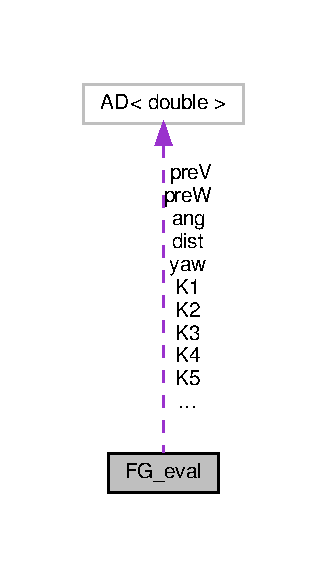
\includegraphics[width=157pt]{classFG__eval__coll__graph}
\end{center}
\end{figure}
\subsection*{Public Member Functions}
\begin{DoxyCompactItemize}
\item 
typedef \hyperlink{classFG__eval_aa996df77a971dedd5d5715ef6be1258e}{C\+P\+P\+A\+D\+\_\+\+T\+E\+S\+T\+V\+E\+C\+T\+OR} (AD$<$ double $>$) A\+Dvector
\item 
\hyperlink{classFG__eval_a0a9e41e75d2ab3597a535a73b2a30ede}{F\+G\+\_\+eval} ()
\item 
\hyperlink{classFG__eval_af179064157f6328d47b2ce44c2d30a3e}{F\+G\+\_\+eval} (double \+\_\+xp, double \+\_\+yp, double \+\_\+ap, double \+\_\+dist, double \+\_\+ang, double \+\_\+yaw, double \+\_\+\+K1, double \+\_\+\+K2, double \+\_\+\+K3, double \+\_\+\+K4, double \+\_\+\+K5, double \+\_\+preV, double \+\_\+preW)
\item 
void \hyperlink{classFG__eval_ae4a15abb127b46d10bca1f1619faf248}{operator()} (A\+Dvector \&fg, const A\+Dvector \&x)
\end{DoxyCompactItemize}
\subsection*{Private Attributes}
\begin{DoxyCompactItemize}
\item 
double \hyperlink{classFG__eval_ae37d43302e8c2f0768e0903afdc4dec5}{xp}
\item 
double \hyperlink{classFG__eval_a8df0b0ddcb354b68551c11a1788a9b6e}{yp}
\item 
double \hyperlink{classFG__eval_a8cea35a0a3b58c8dc7cc9be19a1e9013}{ap}
\item 
AD$<$ double $>$ \hyperlink{classFG__eval_a5dcf5982e81dceca40b4bc474827b5aa}{K1}
\item 
AD$<$ double $>$ \hyperlink{classFG__eval_af671d3c7db3b17c2a6fda4798b402320}{K2}
\item 
AD$<$ double $>$ \hyperlink{classFG__eval_a6afb8dacd318791bdad27da2649ff618}{K3}
\item 
AD$<$ double $>$ \hyperlink{classFG__eval_a45479bca30dc7f49625d0d05fd17bc7c}{K4}
\item 
AD$<$ double $>$ \hyperlink{classFG__eval_a969e08a07221e37ccce7ec008aea7356}{K5}
\item 
AD$<$ double $>$ \hyperlink{classFG__eval_a679badb474e00e9d169f1bdc24657129}{dist}
\item 
AD$<$ double $>$ \hyperlink{classFG__eval_a9e9644f7d9759e9fc3babf41d658cbf7}{ang}
\item 
AD$<$ double $>$ \hyperlink{classFG__eval_a6ce3987053540554a0287422fb4f5ce2}{yaw}
\item 
AD$<$ double $>$ \hyperlink{classFG__eval_ab24a3bc79de568dd46827959993a7dc6}{preV}
\item 
AD$<$ double $>$ \hyperlink{classFG__eval_a2efce268a9d4e915e8cd6f670bf80217}{preW}
\end{DoxyCompactItemize}


\subsection{Constructor \& Destructor Documentation}
\mbox{\Hypertarget{classFG__eval_a0a9e41e75d2ab3597a535a73b2a30ede}\label{classFG__eval_a0a9e41e75d2ab3597a535a73b2a30ede}} 
\index{F\+G\+\_\+eval@{F\+G\+\_\+eval}!F\+G\+\_\+eval@{F\+G\+\_\+eval}}
\index{F\+G\+\_\+eval@{F\+G\+\_\+eval}!F\+G\+\_\+eval@{F\+G\+\_\+eval}}
\subsubsection{\texorpdfstring{F\+G\+\_\+eval()}{FG\_eval()}\hspace{0.1cm}{\footnotesize\ttfamily [1/2]}}
{\footnotesize\ttfamily F\+G\+\_\+eval\+::\+F\+G\+\_\+eval (\begin{DoxyParamCaption}{ }\end{DoxyParamCaption})}

\mbox{\Hypertarget{classFG__eval_af179064157f6328d47b2ce44c2d30a3e}\label{classFG__eval_af179064157f6328d47b2ce44c2d30a3e}} 
\index{F\+G\+\_\+eval@{F\+G\+\_\+eval}!F\+G\+\_\+eval@{F\+G\+\_\+eval}}
\index{F\+G\+\_\+eval@{F\+G\+\_\+eval}!F\+G\+\_\+eval@{F\+G\+\_\+eval}}
\subsubsection{\texorpdfstring{F\+G\+\_\+eval()}{FG\_eval()}\hspace{0.1cm}{\footnotesize\ttfamily [2/2]}}
{\footnotesize\ttfamily F\+G\+\_\+eval\+::\+F\+G\+\_\+eval (\begin{DoxyParamCaption}\item[{double}]{\+\_\+xp,  }\item[{double}]{\+\_\+yp,  }\item[{double}]{\+\_\+ap,  }\item[{double}]{\+\_\+dist,  }\item[{double}]{\+\_\+ang,  }\item[{double}]{\+\_\+yaw,  }\item[{double}]{\+\_\+\+K1,  }\item[{double}]{\+\_\+\+K2,  }\item[{double}]{\+\_\+\+K3,  }\item[{double}]{\+\_\+\+K4,  }\item[{double}]{\+\_\+\+K5,  }\item[{double}]{\+\_\+preV,  }\item[{double}]{\+\_\+preW }\end{DoxyParamCaption})}



\subsection{Member Function Documentation}
\mbox{\Hypertarget{classFG__eval_aa996df77a971dedd5d5715ef6be1258e}\label{classFG__eval_aa996df77a971dedd5d5715ef6be1258e}} 
\index{F\+G\+\_\+eval@{F\+G\+\_\+eval}!C\+P\+P\+A\+D\+\_\+\+T\+E\+S\+T\+V\+E\+C\+T\+OR@{C\+P\+P\+A\+D\+\_\+\+T\+E\+S\+T\+V\+E\+C\+T\+OR}}
\index{C\+P\+P\+A\+D\+\_\+\+T\+E\+S\+T\+V\+E\+C\+T\+OR@{C\+P\+P\+A\+D\+\_\+\+T\+E\+S\+T\+V\+E\+C\+T\+OR}!F\+G\+\_\+eval@{F\+G\+\_\+eval}}
\subsubsection{\texorpdfstring{C\+P\+P\+A\+D\+\_\+\+T\+E\+S\+T\+V\+E\+C\+T\+O\+R()}{CPPAD\_TESTVECTOR()}}
{\footnotesize\ttfamily typedef F\+G\+\_\+eval\+::\+C\+P\+P\+A\+D\+\_\+\+T\+E\+S\+T\+V\+E\+C\+T\+OR (\begin{DoxyParamCaption}\item[{AD$<$ double $>$}]{ }\end{DoxyParamCaption})}

\mbox{\Hypertarget{classFG__eval_ae4a15abb127b46d10bca1f1619faf248}\label{classFG__eval_ae4a15abb127b46d10bca1f1619faf248}} 
\index{F\+G\+\_\+eval@{F\+G\+\_\+eval}!operator()@{operator()}}
\index{operator()@{operator()}!F\+G\+\_\+eval@{F\+G\+\_\+eval}}
\subsubsection{\texorpdfstring{operator()()}{operator()()}}
{\footnotesize\ttfamily void F\+G\+\_\+eval\+::operator() (\begin{DoxyParamCaption}\item[{A\+Dvector \&}]{fg,  }\item[{const A\+Dvector \&}]{x }\end{DoxyParamCaption})}



\subsection{Member Data Documentation}
\mbox{\Hypertarget{classFG__eval_a9e9644f7d9759e9fc3babf41d658cbf7}\label{classFG__eval_a9e9644f7d9759e9fc3babf41d658cbf7}} 
\index{F\+G\+\_\+eval@{F\+G\+\_\+eval}!ang@{ang}}
\index{ang@{ang}!F\+G\+\_\+eval@{F\+G\+\_\+eval}}
\subsubsection{\texorpdfstring{ang}{ang}}
{\footnotesize\ttfamily AD$<$double$>$ F\+G\+\_\+eval\+::ang\hspace{0.3cm}{\ttfamily [private]}}

\mbox{\Hypertarget{classFG__eval_a8cea35a0a3b58c8dc7cc9be19a1e9013}\label{classFG__eval_a8cea35a0a3b58c8dc7cc9be19a1e9013}} 
\index{F\+G\+\_\+eval@{F\+G\+\_\+eval}!ap@{ap}}
\index{ap@{ap}!F\+G\+\_\+eval@{F\+G\+\_\+eval}}
\subsubsection{\texorpdfstring{ap}{ap}}
{\footnotesize\ttfamily double F\+G\+\_\+eval\+::ap\hspace{0.3cm}{\ttfamily [private]}}

\mbox{\Hypertarget{classFG__eval_a679badb474e00e9d169f1bdc24657129}\label{classFG__eval_a679badb474e00e9d169f1bdc24657129}} 
\index{F\+G\+\_\+eval@{F\+G\+\_\+eval}!dist@{dist}}
\index{dist@{dist}!F\+G\+\_\+eval@{F\+G\+\_\+eval}}
\subsubsection{\texorpdfstring{dist}{dist}}
{\footnotesize\ttfamily AD$<$double$>$ F\+G\+\_\+eval\+::dist\hspace{0.3cm}{\ttfamily [private]}}

\mbox{\Hypertarget{classFG__eval_a5dcf5982e81dceca40b4bc474827b5aa}\label{classFG__eval_a5dcf5982e81dceca40b4bc474827b5aa}} 
\index{F\+G\+\_\+eval@{F\+G\+\_\+eval}!K1@{K1}}
\index{K1@{K1}!F\+G\+\_\+eval@{F\+G\+\_\+eval}}
\subsubsection{\texorpdfstring{K1}{K1}}
{\footnotesize\ttfamily AD$<$double$>$ F\+G\+\_\+eval\+::\+K1\hspace{0.3cm}{\ttfamily [private]}}

\mbox{\Hypertarget{classFG__eval_af671d3c7db3b17c2a6fda4798b402320}\label{classFG__eval_af671d3c7db3b17c2a6fda4798b402320}} 
\index{F\+G\+\_\+eval@{F\+G\+\_\+eval}!K2@{K2}}
\index{K2@{K2}!F\+G\+\_\+eval@{F\+G\+\_\+eval}}
\subsubsection{\texorpdfstring{K2}{K2}}
{\footnotesize\ttfamily AD$<$double$>$ F\+G\+\_\+eval\+::\+K2\hspace{0.3cm}{\ttfamily [private]}}

\mbox{\Hypertarget{classFG__eval_a6afb8dacd318791bdad27da2649ff618}\label{classFG__eval_a6afb8dacd318791bdad27da2649ff618}} 
\index{F\+G\+\_\+eval@{F\+G\+\_\+eval}!K3@{K3}}
\index{K3@{K3}!F\+G\+\_\+eval@{F\+G\+\_\+eval}}
\subsubsection{\texorpdfstring{K3}{K3}}
{\footnotesize\ttfamily AD$<$double$>$ F\+G\+\_\+eval\+::\+K3\hspace{0.3cm}{\ttfamily [private]}}

\mbox{\Hypertarget{classFG__eval_a45479bca30dc7f49625d0d05fd17bc7c}\label{classFG__eval_a45479bca30dc7f49625d0d05fd17bc7c}} 
\index{F\+G\+\_\+eval@{F\+G\+\_\+eval}!K4@{K4}}
\index{K4@{K4}!F\+G\+\_\+eval@{F\+G\+\_\+eval}}
\subsubsection{\texorpdfstring{K4}{K4}}
{\footnotesize\ttfamily AD$<$double$>$ F\+G\+\_\+eval\+::\+K4\hspace{0.3cm}{\ttfamily [private]}}

\mbox{\Hypertarget{classFG__eval_a969e08a07221e37ccce7ec008aea7356}\label{classFG__eval_a969e08a07221e37ccce7ec008aea7356}} 
\index{F\+G\+\_\+eval@{F\+G\+\_\+eval}!K5@{K5}}
\index{K5@{K5}!F\+G\+\_\+eval@{F\+G\+\_\+eval}}
\subsubsection{\texorpdfstring{K5}{K5}}
{\footnotesize\ttfamily AD$<$double$>$ F\+G\+\_\+eval\+::\+K5\hspace{0.3cm}{\ttfamily [private]}}

\mbox{\Hypertarget{classFG__eval_ab24a3bc79de568dd46827959993a7dc6}\label{classFG__eval_ab24a3bc79de568dd46827959993a7dc6}} 
\index{F\+G\+\_\+eval@{F\+G\+\_\+eval}!preV@{preV}}
\index{preV@{preV}!F\+G\+\_\+eval@{F\+G\+\_\+eval}}
\subsubsection{\texorpdfstring{preV}{preV}}
{\footnotesize\ttfamily AD$<$double$>$ F\+G\+\_\+eval\+::preV\hspace{0.3cm}{\ttfamily [private]}}

\mbox{\Hypertarget{classFG__eval_a2efce268a9d4e915e8cd6f670bf80217}\label{classFG__eval_a2efce268a9d4e915e8cd6f670bf80217}} 
\index{F\+G\+\_\+eval@{F\+G\+\_\+eval}!preW@{preW}}
\index{preW@{preW}!F\+G\+\_\+eval@{F\+G\+\_\+eval}}
\subsubsection{\texorpdfstring{preW}{preW}}
{\footnotesize\ttfamily AD$<$double$>$ F\+G\+\_\+eval\+::preW\hspace{0.3cm}{\ttfamily [private]}}

\mbox{\Hypertarget{classFG__eval_ae37d43302e8c2f0768e0903afdc4dec5}\label{classFG__eval_ae37d43302e8c2f0768e0903afdc4dec5}} 
\index{F\+G\+\_\+eval@{F\+G\+\_\+eval}!xp@{xp}}
\index{xp@{xp}!F\+G\+\_\+eval@{F\+G\+\_\+eval}}
\subsubsection{\texorpdfstring{xp}{xp}}
{\footnotesize\ttfamily double F\+G\+\_\+eval\+::xp\hspace{0.3cm}{\ttfamily [private]}}

\mbox{\Hypertarget{classFG__eval_a6ce3987053540554a0287422fb4f5ce2}\label{classFG__eval_a6ce3987053540554a0287422fb4f5ce2}} 
\index{F\+G\+\_\+eval@{F\+G\+\_\+eval}!yaw@{yaw}}
\index{yaw@{yaw}!F\+G\+\_\+eval@{F\+G\+\_\+eval}}
\subsubsection{\texorpdfstring{yaw}{yaw}}
{\footnotesize\ttfamily AD$<$double$>$ F\+G\+\_\+eval\+::yaw\hspace{0.3cm}{\ttfamily [private]}}

\mbox{\Hypertarget{classFG__eval_a8df0b0ddcb354b68551c11a1788a9b6e}\label{classFG__eval_a8df0b0ddcb354b68551c11a1788a9b6e}} 
\index{F\+G\+\_\+eval@{F\+G\+\_\+eval}!yp@{yp}}
\index{yp@{yp}!F\+G\+\_\+eval@{F\+G\+\_\+eval}}
\subsubsection{\texorpdfstring{yp}{yp}}
{\footnotesize\ttfamily double F\+G\+\_\+eval\+::yp\hspace{0.3cm}{\ttfamily [private]}}



The documentation for this class was generated from the following files\+:\begin{DoxyCompactItemize}
\item 
/home/inazio/\+T\+F\+G/code/catkin\+\_\+ws/src/mpc\+\_\+node/src/\hyperlink{mynlp_8h}{mynlp.\+h}\item 
/home/inazio/\+T\+F\+G/code/catkin\+\_\+ws/src/mpc\+\_\+node/src/\hyperlink{mynlp_8cpp}{mynlp.\+cpp}\end{DoxyCompactItemize}

\hypertarget{classMpc__node}{}\section{Mpc\+\_\+node Class Reference}
\label{classMpc__node}\index{Mpc\+\_\+node@{Mpc\+\_\+node}}


{\ttfamily \#include $<$mpc\+\_\+node.\+hpp$>$}



Collaboration diagram for Mpc\+\_\+node\+:
\nopagebreak
\begin{figure}[H]
\begin{center}
\leavevmode
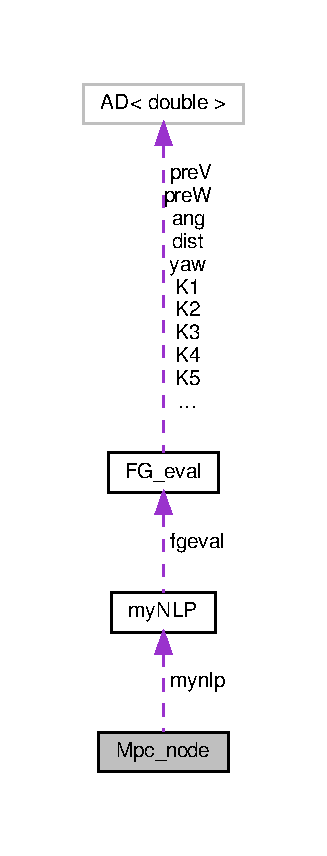
\includegraphics[width=157pt]{classMpc__node__coll__graph}
\end{center}
\end{figure}
\subsection*{Public Member Functions}
\begin{DoxyCompactItemize}
\item 
void \hyperlink{classMpc__node_a708cd33f3a41aac19d767879d1dc0cd7}{pose0\+\_\+callback} (geometry\+\_\+msgs\+::\+Pose\+With\+Covariance\+Stamped pose)
\item 
void \hyperlink{classMpc__node_a4f389e33d9374ed2d18f58125035a0e4}{pose1\+\_\+callback} (geometry\+\_\+msgs\+::\+Pose\+With\+Covariance\+Stamped pose)
\item 
void \hyperlink{classMpc__node_ab55c31f17c32c247adbcee5aae40c128}{calculate\+\_\+fake\+\_\+path} (double \+\_\+xr, double \+\_\+yr, double \+\_\+wr, double \+\_\+xp, double \+\_\+yp, double \+\_\+wp)
\item 
void \hyperlink{classMpc__node_a16734474d794c1896aebd9a008b96611}{publish\+\_\+new\+\_\+path} (tf\+::\+Transform\+Listener $\ast$\hyperlink{classMpc__node_acca5492f6ed78d47688621941d11d1b2}{transform\+\_\+listener}, \hyperlink{classmyNLP}{my\+N\+LP} $\ast$\hyperlink{classMpc__node_a5a7534e2aaa1e1003d4c710589e07590}{mynlp})
\item 
void \hyperlink{classMpc__node_a97467f6ef0d64235da935823cfd4bd47}{publish\+\_\+new\+\_\+actions} (\hyperlink{classmyNLP}{my\+N\+LP} $\ast$\hyperlink{classMpc__node_a5a7534e2aaa1e1003d4c710589e07590}{mynlp})
\item 
void \hyperlink{classMpc__node_ab607a3c4dfa4ebf571a60c93049e3309}{get\+\_\+parameters} ()
\item 
void \hyperlink{classMpc__node_a788f17ed756892727cf04adf1a485677}{control\+\_\+loop} ()
\item 
\hyperlink{classMpc__node_aecd75162dde3b8750c37e0b85a036097}{Mpc\+\_\+node} ()
\end{DoxyCompactItemize}
\subsection*{Private Attributes}
\begin{DoxyCompactItemize}
\item 
ros\+::\+Node\+Handle \hyperlink{classMpc__node_a6d876c2baef47329ce66b8747b918eb4}{n}
\item 
ros\+::\+Rate \hyperlink{classMpc__node_accb78ea73903c0a6164b794d0450a0b0}{rate}
\item 
ros\+::\+Publisher \hyperlink{classMpc__node_a4c51498e7db8875e951c637e891b5e62}{pub\+Path}
\item 
ros\+::\+Publisher \hyperlink{classMpc__node_a4191433cb5c29c422a6ac11abfb2c08f}{pubV}
\item 
ros\+::\+Subscriber \hyperlink{classMpc__node_a97fdf7b8912632aac250aeb4a515d38f}{sub\+Pose0}
\item 
ros\+::\+Subscriber \hyperlink{classMpc__node_aec569d4ea7254ec9893ce79b94ce2eba}{sub\+Pose1}
\item 
tf\+::\+Transform\+Listener \hyperlink{classMpc__node_acca5492f6ed78d47688621941d11d1b2}{transform\+\_\+listener}
\item 
tf\+::\+Stamped\+Transform \hyperlink{classMpc__node_a8688cf07e5ddc56acf1448503b3f5984}{R\+T\+\_\+person\+\_\+robot}
\item 
ros\+::\+Time \hyperlink{classMpc__node_a5412f969d238133ee5a5a40928811932}{time\+\_\+start}
\item 
nav\+\_\+msgs\+::\+Path \hyperlink{classMpc__node_a6da2728783a52910d4c378a3f66aec06}{path}
\item 
double \hyperlink{classMpc__node_a28803c0f092db658637ece996aad7e90}{dist} = 3.\+0
\item 
double \hyperlink{classMpc__node_a44c011b9b0c84002f5e9cb057c9a2d59}{ang} = 0.\+0
\item 
double \hyperlink{classMpc__node_a9b5da0aaf367d5b1f60f47eca976de2a}{yaw} = -\/1.\+57
\item 
double \hyperlink{classMpc__node_a5c4d6221612047ebd47b0c0fe462db67}{K1} = 1.\+0
\item 
double \hyperlink{classMpc__node_a78c903e351af27fd9e4b92c2a4d40210}{K2} = 1.\+0
\item 
double \hyperlink{classMpc__node_a4a889c942598f48d5ec29f45e7c98478}{K3} = 1.\+0
\item 
double \hyperlink{classMpc__node_a0b2df940218a00cdfbedb434bb108d5a}{K4} = 0.\+5
\item 
double \hyperlink{classMpc__node_a893fd885d574e00cbe38cbcd06079aca}{K5} = 0.\+5
\item 
double \hyperlink{classMpc__node_a1d0e857050592ddf6afa764a74a03f4a}{vmax} = 1.\+5
\item 
double \hyperlink{classMpc__node_a85d68b460b951590985a52dabdb0ba4b}{wmax} = 0.\+78
\item 
bool \hyperlink{classMpc__node_a4ac01e38cecc492097d9fabd33afab8d}{use\+Ground\+Truth} = false
\item 
\hyperlink{classmyNLP}{my\+N\+LP} \hyperlink{classMpc__node_a5a7534e2aaa1e1003d4c710589e07590}{mynlp}
\item 
double \hyperlink{classMpc__node_a5e3e13f0270d4e8c3555c60a3a9b5356}{xr}
\item 
double \hyperlink{classMpc__node_a93c8464ce2e0446c7463bad6a52ee8a1}{yr}
\item 
double \hyperlink{classMpc__node_a78f2cb060ecee1c0be22b9b59fb0638e}{titar}
\item 
double \hyperlink{classMpc__node_aeb6d97153be787995ddefaa9839e09c0}{xp}
\item 
double \hyperlink{classMpc__node_adb9780e9f20aa698a68fbc632b8e4f46}{yp}
\item 
double \hyperlink{classMpc__node_ad599feb3182645b6359b6bb16055fcb8}{titap}
\end{DoxyCompactItemize}


\subsection{Constructor \& Destructor Documentation}
\mbox{\Hypertarget{classMpc__node_aecd75162dde3b8750c37e0b85a036097}\label{classMpc__node_aecd75162dde3b8750c37e0b85a036097}} 
\index{Mpc\+\_\+node@{Mpc\+\_\+node}!Mpc\+\_\+node@{Mpc\+\_\+node}}
\index{Mpc\+\_\+node@{Mpc\+\_\+node}!Mpc\+\_\+node@{Mpc\+\_\+node}}
\subsubsection{\texorpdfstring{Mpc\+\_\+node()}{Mpc\_node()}}
{\footnotesize\ttfamily Mpc\+\_\+node\+::\+Mpc\+\_\+node (\begin{DoxyParamCaption}{ }\end{DoxyParamCaption})}



\subsection{Member Function Documentation}
\mbox{\Hypertarget{classMpc__node_ab55c31f17c32c247adbcee5aae40c128}\label{classMpc__node_ab55c31f17c32c247adbcee5aae40c128}} 
\index{Mpc\+\_\+node@{Mpc\+\_\+node}!calculate\+\_\+fake\+\_\+path@{calculate\+\_\+fake\+\_\+path}}
\index{calculate\+\_\+fake\+\_\+path@{calculate\+\_\+fake\+\_\+path}!Mpc\+\_\+node@{Mpc\+\_\+node}}
\subsubsection{\texorpdfstring{calculate\+\_\+fake\+\_\+path()}{calculate\_fake\_path()}}
{\footnotesize\ttfamily void Mpc\+\_\+node\+::calculate\+\_\+fake\+\_\+path (\begin{DoxyParamCaption}\item[{double}]{\+\_\+xr,  }\item[{double}]{\+\_\+yr,  }\item[{double}]{\+\_\+wr,  }\item[{double}]{\+\_\+xp,  }\item[{double}]{\+\_\+yp,  }\item[{double}]{\+\_\+wp }\end{DoxyParamCaption})}

\mbox{\Hypertarget{classMpc__node_a788f17ed756892727cf04adf1a485677}\label{classMpc__node_a788f17ed756892727cf04adf1a485677}} 
\index{Mpc\+\_\+node@{Mpc\+\_\+node}!control\+\_\+loop@{control\+\_\+loop}}
\index{control\+\_\+loop@{control\+\_\+loop}!Mpc\+\_\+node@{Mpc\+\_\+node}}
\subsubsection{\texorpdfstring{control\+\_\+loop()}{control\_loop()}}
{\footnotesize\ttfamily void Mpc\+\_\+node\+::control\+\_\+loop (\begin{DoxyParamCaption}{ }\end{DoxyParamCaption})}

\mbox{\Hypertarget{classMpc__node_ab607a3c4dfa4ebf571a60c93049e3309}\label{classMpc__node_ab607a3c4dfa4ebf571a60c93049e3309}} 
\index{Mpc\+\_\+node@{Mpc\+\_\+node}!get\+\_\+parameters@{get\+\_\+parameters}}
\index{get\+\_\+parameters@{get\+\_\+parameters}!Mpc\+\_\+node@{Mpc\+\_\+node}}
\subsubsection{\texorpdfstring{get\+\_\+parameters()}{get\_parameters()}}
{\footnotesize\ttfamily void Mpc\+\_\+node\+::get\+\_\+parameters (\begin{DoxyParamCaption}{ }\end{DoxyParamCaption})}

\mbox{\Hypertarget{classMpc__node_a708cd33f3a41aac19d767879d1dc0cd7}\label{classMpc__node_a708cd33f3a41aac19d767879d1dc0cd7}} 
\index{Mpc\+\_\+node@{Mpc\+\_\+node}!pose0\+\_\+callback@{pose0\+\_\+callback}}
\index{pose0\+\_\+callback@{pose0\+\_\+callback}!Mpc\+\_\+node@{Mpc\+\_\+node}}
\subsubsection{\texorpdfstring{pose0\+\_\+callback()}{pose0\_callback()}}
{\footnotesize\ttfamily void Mpc\+\_\+node\+::pose0\+\_\+callback (\begin{DoxyParamCaption}\item[{geometry\+\_\+msgs\+::\+Pose\+With\+Covariance\+Stamped}]{pose }\end{DoxyParamCaption})}

\mbox{\Hypertarget{classMpc__node_a4f389e33d9374ed2d18f58125035a0e4}\label{classMpc__node_a4f389e33d9374ed2d18f58125035a0e4}} 
\index{Mpc\+\_\+node@{Mpc\+\_\+node}!pose1\+\_\+callback@{pose1\+\_\+callback}}
\index{pose1\+\_\+callback@{pose1\+\_\+callback}!Mpc\+\_\+node@{Mpc\+\_\+node}}
\subsubsection{\texorpdfstring{pose1\+\_\+callback()}{pose1\_callback()}}
{\footnotesize\ttfamily void Mpc\+\_\+node\+::pose1\+\_\+callback (\begin{DoxyParamCaption}\item[{geometry\+\_\+msgs\+::\+Pose\+With\+Covariance\+Stamped}]{pose }\end{DoxyParamCaption})}

\mbox{\Hypertarget{classMpc__node_a97467f6ef0d64235da935823cfd4bd47}\label{classMpc__node_a97467f6ef0d64235da935823cfd4bd47}} 
\index{Mpc\+\_\+node@{Mpc\+\_\+node}!publish\+\_\+new\+\_\+actions@{publish\+\_\+new\+\_\+actions}}
\index{publish\+\_\+new\+\_\+actions@{publish\+\_\+new\+\_\+actions}!Mpc\+\_\+node@{Mpc\+\_\+node}}
\subsubsection{\texorpdfstring{publish\+\_\+new\+\_\+actions()}{publish\_new\_actions()}}
{\footnotesize\ttfamily void Mpc\+\_\+node\+::publish\+\_\+new\+\_\+actions (\begin{DoxyParamCaption}\item[{\hyperlink{classmyNLP}{my\+N\+LP} $\ast$}]{mynlp }\end{DoxyParamCaption})}

\mbox{\Hypertarget{classMpc__node_a16734474d794c1896aebd9a008b96611}\label{classMpc__node_a16734474d794c1896aebd9a008b96611}} 
\index{Mpc\+\_\+node@{Mpc\+\_\+node}!publish\+\_\+new\+\_\+path@{publish\+\_\+new\+\_\+path}}
\index{publish\+\_\+new\+\_\+path@{publish\+\_\+new\+\_\+path}!Mpc\+\_\+node@{Mpc\+\_\+node}}
\subsubsection{\texorpdfstring{publish\+\_\+new\+\_\+path()}{publish\_new\_path()}}
{\footnotesize\ttfamily void Mpc\+\_\+node\+::publish\+\_\+new\+\_\+path (\begin{DoxyParamCaption}\item[{tf\+::\+Transform\+Listener $\ast$}]{transform\+\_\+listener,  }\item[{\hyperlink{classmyNLP}{my\+N\+LP} $\ast$}]{mynlp }\end{DoxyParamCaption})}



\subsection{Member Data Documentation}
\mbox{\Hypertarget{classMpc__node_a44c011b9b0c84002f5e9cb057c9a2d59}\label{classMpc__node_a44c011b9b0c84002f5e9cb057c9a2d59}} 
\index{Mpc\+\_\+node@{Mpc\+\_\+node}!ang@{ang}}
\index{ang@{ang}!Mpc\+\_\+node@{Mpc\+\_\+node}}
\subsubsection{\texorpdfstring{ang}{ang}}
{\footnotesize\ttfamily double Mpc\+\_\+node\+::ang = 0.\+0\hspace{0.3cm}{\ttfamily [private]}}

\mbox{\Hypertarget{classMpc__node_a28803c0f092db658637ece996aad7e90}\label{classMpc__node_a28803c0f092db658637ece996aad7e90}} 
\index{Mpc\+\_\+node@{Mpc\+\_\+node}!dist@{dist}}
\index{dist@{dist}!Mpc\+\_\+node@{Mpc\+\_\+node}}
\subsubsection{\texorpdfstring{dist}{dist}}
{\footnotesize\ttfamily double Mpc\+\_\+node\+::dist = 3.\+0\hspace{0.3cm}{\ttfamily [private]}}

\mbox{\Hypertarget{classMpc__node_a5c4d6221612047ebd47b0c0fe462db67}\label{classMpc__node_a5c4d6221612047ebd47b0c0fe462db67}} 
\index{Mpc\+\_\+node@{Mpc\+\_\+node}!K1@{K1}}
\index{K1@{K1}!Mpc\+\_\+node@{Mpc\+\_\+node}}
\subsubsection{\texorpdfstring{K1}{K1}}
{\footnotesize\ttfamily double Mpc\+\_\+node\+::\+K1 = 1.\+0\hspace{0.3cm}{\ttfamily [private]}}

\mbox{\Hypertarget{classMpc__node_a78c903e351af27fd9e4b92c2a4d40210}\label{classMpc__node_a78c903e351af27fd9e4b92c2a4d40210}} 
\index{Mpc\+\_\+node@{Mpc\+\_\+node}!K2@{K2}}
\index{K2@{K2}!Mpc\+\_\+node@{Mpc\+\_\+node}}
\subsubsection{\texorpdfstring{K2}{K2}}
{\footnotesize\ttfamily double Mpc\+\_\+node\+::\+K2 = 1.\+0\hspace{0.3cm}{\ttfamily [private]}}

\mbox{\Hypertarget{classMpc__node_a4a889c942598f48d5ec29f45e7c98478}\label{classMpc__node_a4a889c942598f48d5ec29f45e7c98478}} 
\index{Mpc\+\_\+node@{Mpc\+\_\+node}!K3@{K3}}
\index{K3@{K3}!Mpc\+\_\+node@{Mpc\+\_\+node}}
\subsubsection{\texorpdfstring{K3}{K3}}
{\footnotesize\ttfamily double Mpc\+\_\+node\+::\+K3 = 1.\+0\hspace{0.3cm}{\ttfamily [private]}}

\mbox{\Hypertarget{classMpc__node_a0b2df940218a00cdfbedb434bb108d5a}\label{classMpc__node_a0b2df940218a00cdfbedb434bb108d5a}} 
\index{Mpc\+\_\+node@{Mpc\+\_\+node}!K4@{K4}}
\index{K4@{K4}!Mpc\+\_\+node@{Mpc\+\_\+node}}
\subsubsection{\texorpdfstring{K4}{K4}}
{\footnotesize\ttfamily double Mpc\+\_\+node\+::\+K4 = 0.\+5\hspace{0.3cm}{\ttfamily [private]}}

\mbox{\Hypertarget{classMpc__node_a893fd885d574e00cbe38cbcd06079aca}\label{classMpc__node_a893fd885d574e00cbe38cbcd06079aca}} 
\index{Mpc\+\_\+node@{Mpc\+\_\+node}!K5@{K5}}
\index{K5@{K5}!Mpc\+\_\+node@{Mpc\+\_\+node}}
\subsubsection{\texorpdfstring{K5}{K5}}
{\footnotesize\ttfamily double Mpc\+\_\+node\+::\+K5 = 0.\+5\hspace{0.3cm}{\ttfamily [private]}}

\mbox{\Hypertarget{classMpc__node_a5a7534e2aaa1e1003d4c710589e07590}\label{classMpc__node_a5a7534e2aaa1e1003d4c710589e07590}} 
\index{Mpc\+\_\+node@{Mpc\+\_\+node}!mynlp@{mynlp}}
\index{mynlp@{mynlp}!Mpc\+\_\+node@{Mpc\+\_\+node}}
\subsubsection{\texorpdfstring{mynlp}{mynlp}}
{\footnotesize\ttfamily \hyperlink{classmyNLP}{my\+N\+LP} Mpc\+\_\+node\+::mynlp\hspace{0.3cm}{\ttfamily [private]}}

\mbox{\Hypertarget{classMpc__node_a6d876c2baef47329ce66b8747b918eb4}\label{classMpc__node_a6d876c2baef47329ce66b8747b918eb4}} 
\index{Mpc\+\_\+node@{Mpc\+\_\+node}!n@{n}}
\index{n@{n}!Mpc\+\_\+node@{Mpc\+\_\+node}}
\subsubsection{\texorpdfstring{n}{n}}
{\footnotesize\ttfamily ros\+::\+Node\+Handle Mpc\+\_\+node\+::n\hspace{0.3cm}{\ttfamily [private]}}

\mbox{\Hypertarget{classMpc__node_a6da2728783a52910d4c378a3f66aec06}\label{classMpc__node_a6da2728783a52910d4c378a3f66aec06}} 
\index{Mpc\+\_\+node@{Mpc\+\_\+node}!path@{path}}
\index{path@{path}!Mpc\+\_\+node@{Mpc\+\_\+node}}
\subsubsection{\texorpdfstring{path}{path}}
{\footnotesize\ttfamily nav\+\_\+msgs\+::\+Path Mpc\+\_\+node\+::path\hspace{0.3cm}{\ttfamily [private]}}

\mbox{\Hypertarget{classMpc__node_a4c51498e7db8875e951c637e891b5e62}\label{classMpc__node_a4c51498e7db8875e951c637e891b5e62}} 
\index{Mpc\+\_\+node@{Mpc\+\_\+node}!pub\+Path@{pub\+Path}}
\index{pub\+Path@{pub\+Path}!Mpc\+\_\+node@{Mpc\+\_\+node}}
\subsubsection{\texorpdfstring{pub\+Path}{pubPath}}
{\footnotesize\ttfamily ros\+::\+Publisher Mpc\+\_\+node\+::pub\+Path\hspace{0.3cm}{\ttfamily [private]}}

\mbox{\Hypertarget{classMpc__node_a4191433cb5c29c422a6ac11abfb2c08f}\label{classMpc__node_a4191433cb5c29c422a6ac11abfb2c08f}} 
\index{Mpc\+\_\+node@{Mpc\+\_\+node}!pubV@{pubV}}
\index{pubV@{pubV}!Mpc\+\_\+node@{Mpc\+\_\+node}}
\subsubsection{\texorpdfstring{pubV}{pubV}}
{\footnotesize\ttfamily ros\+::\+Publisher Mpc\+\_\+node\+::pubV\hspace{0.3cm}{\ttfamily [private]}}

\mbox{\Hypertarget{classMpc__node_accb78ea73903c0a6164b794d0450a0b0}\label{classMpc__node_accb78ea73903c0a6164b794d0450a0b0}} 
\index{Mpc\+\_\+node@{Mpc\+\_\+node}!rate@{rate}}
\index{rate@{rate}!Mpc\+\_\+node@{Mpc\+\_\+node}}
\subsubsection{\texorpdfstring{rate}{rate}}
{\footnotesize\ttfamily ros\+::\+Rate Mpc\+\_\+node\+::rate\hspace{0.3cm}{\ttfamily [private]}}

\mbox{\Hypertarget{classMpc__node_a8688cf07e5ddc56acf1448503b3f5984}\label{classMpc__node_a8688cf07e5ddc56acf1448503b3f5984}} 
\index{Mpc\+\_\+node@{Mpc\+\_\+node}!R\+T\+\_\+person\+\_\+robot@{R\+T\+\_\+person\+\_\+robot}}
\index{R\+T\+\_\+person\+\_\+robot@{R\+T\+\_\+person\+\_\+robot}!Mpc\+\_\+node@{Mpc\+\_\+node}}
\subsubsection{\texorpdfstring{R\+T\+\_\+person\+\_\+robot}{RT\_person\_robot}}
{\footnotesize\ttfamily tf\+::\+Stamped\+Transform Mpc\+\_\+node\+::\+R\+T\+\_\+person\+\_\+robot\hspace{0.3cm}{\ttfamily [private]}}

\mbox{\Hypertarget{classMpc__node_a97fdf7b8912632aac250aeb4a515d38f}\label{classMpc__node_a97fdf7b8912632aac250aeb4a515d38f}} 
\index{Mpc\+\_\+node@{Mpc\+\_\+node}!sub\+Pose0@{sub\+Pose0}}
\index{sub\+Pose0@{sub\+Pose0}!Mpc\+\_\+node@{Mpc\+\_\+node}}
\subsubsection{\texorpdfstring{sub\+Pose0}{subPose0}}
{\footnotesize\ttfamily ros\+::\+Subscriber Mpc\+\_\+node\+::sub\+Pose0\hspace{0.3cm}{\ttfamily [private]}}

\mbox{\Hypertarget{classMpc__node_aec569d4ea7254ec9893ce79b94ce2eba}\label{classMpc__node_aec569d4ea7254ec9893ce79b94ce2eba}} 
\index{Mpc\+\_\+node@{Mpc\+\_\+node}!sub\+Pose1@{sub\+Pose1}}
\index{sub\+Pose1@{sub\+Pose1}!Mpc\+\_\+node@{Mpc\+\_\+node}}
\subsubsection{\texorpdfstring{sub\+Pose1}{subPose1}}
{\footnotesize\ttfamily ros\+::\+Subscriber Mpc\+\_\+node\+::sub\+Pose1\hspace{0.3cm}{\ttfamily [private]}}

\mbox{\Hypertarget{classMpc__node_a5412f969d238133ee5a5a40928811932}\label{classMpc__node_a5412f969d238133ee5a5a40928811932}} 
\index{Mpc\+\_\+node@{Mpc\+\_\+node}!time\+\_\+start@{time\+\_\+start}}
\index{time\+\_\+start@{time\+\_\+start}!Mpc\+\_\+node@{Mpc\+\_\+node}}
\subsubsection{\texorpdfstring{time\+\_\+start}{time\_start}}
{\footnotesize\ttfamily ros\+::\+Time Mpc\+\_\+node\+::time\+\_\+start\hspace{0.3cm}{\ttfamily [private]}}

\mbox{\Hypertarget{classMpc__node_ad599feb3182645b6359b6bb16055fcb8}\label{classMpc__node_ad599feb3182645b6359b6bb16055fcb8}} 
\index{Mpc\+\_\+node@{Mpc\+\_\+node}!titap@{titap}}
\index{titap@{titap}!Mpc\+\_\+node@{Mpc\+\_\+node}}
\subsubsection{\texorpdfstring{titap}{titap}}
{\footnotesize\ttfamily double Mpc\+\_\+node\+::titap\hspace{0.3cm}{\ttfamily [private]}}

\mbox{\Hypertarget{classMpc__node_a78f2cb060ecee1c0be22b9b59fb0638e}\label{classMpc__node_a78f2cb060ecee1c0be22b9b59fb0638e}} 
\index{Mpc\+\_\+node@{Mpc\+\_\+node}!titar@{titar}}
\index{titar@{titar}!Mpc\+\_\+node@{Mpc\+\_\+node}}
\subsubsection{\texorpdfstring{titar}{titar}}
{\footnotesize\ttfamily double Mpc\+\_\+node\+::titar\hspace{0.3cm}{\ttfamily [private]}}

\mbox{\Hypertarget{classMpc__node_acca5492f6ed78d47688621941d11d1b2}\label{classMpc__node_acca5492f6ed78d47688621941d11d1b2}} 
\index{Mpc\+\_\+node@{Mpc\+\_\+node}!transform\+\_\+listener@{transform\+\_\+listener}}
\index{transform\+\_\+listener@{transform\+\_\+listener}!Mpc\+\_\+node@{Mpc\+\_\+node}}
\subsubsection{\texorpdfstring{transform\+\_\+listener}{transform\_listener}}
{\footnotesize\ttfamily tf\+::\+Transform\+Listener Mpc\+\_\+node\+::transform\+\_\+listener\hspace{0.3cm}{\ttfamily [private]}}

\mbox{\Hypertarget{classMpc__node_a4ac01e38cecc492097d9fabd33afab8d}\label{classMpc__node_a4ac01e38cecc492097d9fabd33afab8d}} 
\index{Mpc\+\_\+node@{Mpc\+\_\+node}!use\+Ground\+Truth@{use\+Ground\+Truth}}
\index{use\+Ground\+Truth@{use\+Ground\+Truth}!Mpc\+\_\+node@{Mpc\+\_\+node}}
\subsubsection{\texorpdfstring{use\+Ground\+Truth}{useGroundTruth}}
{\footnotesize\ttfamily bool Mpc\+\_\+node\+::use\+Ground\+Truth = false\hspace{0.3cm}{\ttfamily [private]}}

\mbox{\Hypertarget{classMpc__node_a1d0e857050592ddf6afa764a74a03f4a}\label{classMpc__node_a1d0e857050592ddf6afa764a74a03f4a}} 
\index{Mpc\+\_\+node@{Mpc\+\_\+node}!vmax@{vmax}}
\index{vmax@{vmax}!Mpc\+\_\+node@{Mpc\+\_\+node}}
\subsubsection{\texorpdfstring{vmax}{vmax}}
{\footnotesize\ttfamily double Mpc\+\_\+node\+::vmax = 1.\+5\hspace{0.3cm}{\ttfamily [private]}}

\mbox{\Hypertarget{classMpc__node_a85d68b460b951590985a52dabdb0ba4b}\label{classMpc__node_a85d68b460b951590985a52dabdb0ba4b}} 
\index{Mpc\+\_\+node@{Mpc\+\_\+node}!wmax@{wmax}}
\index{wmax@{wmax}!Mpc\+\_\+node@{Mpc\+\_\+node}}
\subsubsection{\texorpdfstring{wmax}{wmax}}
{\footnotesize\ttfamily double Mpc\+\_\+node\+::wmax = 0.\+78\hspace{0.3cm}{\ttfamily [private]}}

\mbox{\Hypertarget{classMpc__node_aeb6d97153be787995ddefaa9839e09c0}\label{classMpc__node_aeb6d97153be787995ddefaa9839e09c0}} 
\index{Mpc\+\_\+node@{Mpc\+\_\+node}!xp@{xp}}
\index{xp@{xp}!Mpc\+\_\+node@{Mpc\+\_\+node}}
\subsubsection{\texorpdfstring{xp}{xp}}
{\footnotesize\ttfamily double Mpc\+\_\+node\+::xp\hspace{0.3cm}{\ttfamily [private]}}

\mbox{\Hypertarget{classMpc__node_a5e3e13f0270d4e8c3555c60a3a9b5356}\label{classMpc__node_a5e3e13f0270d4e8c3555c60a3a9b5356}} 
\index{Mpc\+\_\+node@{Mpc\+\_\+node}!xr@{xr}}
\index{xr@{xr}!Mpc\+\_\+node@{Mpc\+\_\+node}}
\subsubsection{\texorpdfstring{xr}{xr}}
{\footnotesize\ttfamily double Mpc\+\_\+node\+::xr\hspace{0.3cm}{\ttfamily [private]}}

\mbox{\Hypertarget{classMpc__node_a9b5da0aaf367d5b1f60f47eca976de2a}\label{classMpc__node_a9b5da0aaf367d5b1f60f47eca976de2a}} 
\index{Mpc\+\_\+node@{Mpc\+\_\+node}!yaw@{yaw}}
\index{yaw@{yaw}!Mpc\+\_\+node@{Mpc\+\_\+node}}
\subsubsection{\texorpdfstring{yaw}{yaw}}
{\footnotesize\ttfamily double Mpc\+\_\+node\+::yaw = -\/1.\+57\hspace{0.3cm}{\ttfamily [private]}}

\mbox{\Hypertarget{classMpc__node_adb9780e9f20aa698a68fbc632b8e4f46}\label{classMpc__node_adb9780e9f20aa698a68fbc632b8e4f46}} 
\index{Mpc\+\_\+node@{Mpc\+\_\+node}!yp@{yp}}
\index{yp@{yp}!Mpc\+\_\+node@{Mpc\+\_\+node}}
\subsubsection{\texorpdfstring{yp}{yp}}
{\footnotesize\ttfamily double Mpc\+\_\+node\+::yp\hspace{0.3cm}{\ttfamily [private]}}

\mbox{\Hypertarget{classMpc__node_a93c8464ce2e0446c7463bad6a52ee8a1}\label{classMpc__node_a93c8464ce2e0446c7463bad6a52ee8a1}} 
\index{Mpc\+\_\+node@{Mpc\+\_\+node}!yr@{yr}}
\index{yr@{yr}!Mpc\+\_\+node@{Mpc\+\_\+node}}
\subsubsection{\texorpdfstring{yr}{yr}}
{\footnotesize\ttfamily double Mpc\+\_\+node\+::yr\hspace{0.3cm}{\ttfamily [private]}}



The documentation for this class was generated from the following files\+:\begin{DoxyCompactItemize}
\item 
/home/inazio/\+T\+F\+G/code/catkin\+\_\+ws/src/mpc\+\_\+node/src/\hyperlink{mpc__node_8hpp}{mpc\+\_\+node.\+hpp}\item 
/home/inazio/\+T\+F\+G/code/catkin\+\_\+ws/src/mpc\+\_\+node/src/\hyperlink{mpc__node_8cpp}{mpc\+\_\+node.\+cpp}\end{DoxyCompactItemize}

\hypertarget{classmyNLP}{}\section{my\+N\+LP Class Reference}
\label{classmyNLP}\index{my\+N\+LP@{my\+N\+LP}}


{\ttfamily \#include $<$mynlp.\+h$>$}



Collaboration diagram for my\+N\+LP\+:
\nopagebreak
\begin{figure}[H]
\begin{center}
\leavevmode
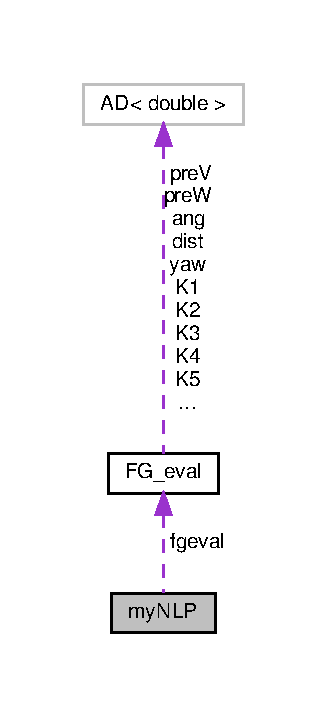
\includegraphics[width=157pt]{classmyNLP__coll__graph}
\end{center}
\end{figure}
\subsection*{Public Member Functions}
\begin{DoxyCompactItemize}
\item 
\hyperlink{classmyNLP_afc4d8a138c3bfbae32449c4360ef4b16}{my\+N\+LP} (double \+\_\+vmax, double \+\_\+wmax)
\item 
void \hyperlink{classmyNLP_ad8eba55aefb5ece257f2c6959aef3f91}{my\+\_\+solve} (double xp, double yp, double ap, double dist, double ang, double yaw, double K1, double K2, double K3, double K4, double K5)
\item 
void \hyperlink{classmyNLP_a71acace73426061aef73e43f31396efa}{save\+\_\+solution} (Cpp\+A\+D\+::ipopt\+::solve\+\_\+result$<$ Dvector $>$ \hyperlink{classmyNLP_ab56c3a82e2b58faa2278143b0d014ff2}{solution})
\end{DoxyCompactItemize}
\subsection*{Public Attributes}
\begin{DoxyCompactItemize}
\item 
std\+::vector$<$ double $>$ \hyperlink{classmyNLP_a723f46ade7987968c50f5b1dc4044bc8}{Xr}
\item 
std\+::vector$<$ double $>$ \hyperlink{classmyNLP_af981a9af6b17e3b406faf365898cfd10}{Yr}
\item 
std\+::vector$<$ double $>$ \hyperlink{classmyNLP_aefab14beb6186061e423865d05645c78}{Titar}
\item 
std\+::vector$<$ double $>$ \hyperlink{classmyNLP_aeea9f95bdd67cf56e2ec2a79944a3cb9}{Vr}
\item 
std\+::vector$<$ double $>$ \hyperlink{classmyNLP_aa3176f5469491b6432f6da85a426957e}{Wr}
\end{DoxyCompactItemize}
\subsection*{Private Attributes}
\begin{DoxyCompactItemize}
\item 
double \hyperlink{classmyNLP_a1ae02d6ab35595595e960b8571558425}{vmax}
\item 
double \hyperlink{classmyNLP_afc3c8ef8ab19ef14565825f779ae104c}{wmax}
\item 
\hyperlink{classFG__eval}{F\+G\+\_\+eval} \hyperlink{classmyNLP_ab8a19e8b3a951c8c7dbe8aad6e3ef270}{fgeval}
\item 
double \hyperlink{classmyNLP_ad357ad6cc7784e3285cfa90b6dc2cc2e}{preV}
\item 
double \hyperlink{classmyNLP_a79269c0f690c30c3127f1453838b72ba}{preW}
\item 
Cpp\+A\+D\+::ipopt\+::solve\+\_\+result$<$ Dvector $>$ \hyperlink{classmyNLP_ab56c3a82e2b58faa2278143b0d014ff2}{solution}
\item 
double \hyperlink{classmyNLP_a99c70b6afb9e1147bbff6da0d58067ec}{av} = 1$\ast$0.\+1
\item 
double \hyperlink{classmyNLP_ae6e75bd5ed3daab0b9d329aed9908095}{aw} = 1$\ast$0.\+1
\end{DoxyCompactItemize}


\subsection{Constructor \& Destructor Documentation}
\mbox{\Hypertarget{classmyNLP_afc4d8a138c3bfbae32449c4360ef4b16}\label{classmyNLP_afc4d8a138c3bfbae32449c4360ef4b16}} 
\index{my\+N\+LP@{my\+N\+LP}!my\+N\+LP@{my\+N\+LP}}
\index{my\+N\+LP@{my\+N\+LP}!my\+N\+LP@{my\+N\+LP}}
\subsubsection{\texorpdfstring{my\+N\+L\+P()}{myNLP()}}
{\footnotesize\ttfamily my\+N\+L\+P\+::my\+N\+LP (\begin{DoxyParamCaption}\item[{double}]{\+\_\+vmax,  }\item[{double}]{\+\_\+wmax }\end{DoxyParamCaption})}



\subsection{Member Function Documentation}
\mbox{\Hypertarget{classmyNLP_ad8eba55aefb5ece257f2c6959aef3f91}\label{classmyNLP_ad8eba55aefb5ece257f2c6959aef3f91}} 
\index{my\+N\+LP@{my\+N\+LP}!my\+\_\+solve@{my\+\_\+solve}}
\index{my\+\_\+solve@{my\+\_\+solve}!my\+N\+LP@{my\+N\+LP}}
\subsubsection{\texorpdfstring{my\+\_\+solve()}{my\_solve()}}
{\footnotesize\ttfamily void my\+N\+L\+P\+::my\+\_\+solve (\begin{DoxyParamCaption}\item[{double}]{xp,  }\item[{double}]{yp,  }\item[{double}]{ap,  }\item[{double}]{dist,  }\item[{double}]{ang,  }\item[{double}]{yaw,  }\item[{double}]{K1,  }\item[{double}]{K2,  }\item[{double}]{K3,  }\item[{double}]{K4,  }\item[{double}]{K5 }\end{DoxyParamCaption})}

\mbox{\Hypertarget{classmyNLP_a71acace73426061aef73e43f31396efa}\label{classmyNLP_a71acace73426061aef73e43f31396efa}} 
\index{my\+N\+LP@{my\+N\+LP}!save\+\_\+solution@{save\+\_\+solution}}
\index{save\+\_\+solution@{save\+\_\+solution}!my\+N\+LP@{my\+N\+LP}}
\subsubsection{\texorpdfstring{save\+\_\+solution()}{save\_solution()}}
{\footnotesize\ttfamily void my\+N\+L\+P\+::save\+\_\+solution (\begin{DoxyParamCaption}\item[{Cpp\+A\+D\+::ipopt\+::solve\+\_\+result$<$ Dvector $>$}]{solution }\end{DoxyParamCaption})}



\subsection{Member Data Documentation}
\mbox{\Hypertarget{classmyNLP_a99c70b6afb9e1147bbff6da0d58067ec}\label{classmyNLP_a99c70b6afb9e1147bbff6da0d58067ec}} 
\index{my\+N\+LP@{my\+N\+LP}!av@{av}}
\index{av@{av}!my\+N\+LP@{my\+N\+LP}}
\subsubsection{\texorpdfstring{av}{av}}
{\footnotesize\ttfamily double my\+N\+L\+P\+::av = 1$\ast$0.\+1\hspace{0.3cm}{\ttfamily [private]}}

\mbox{\Hypertarget{classmyNLP_ae6e75bd5ed3daab0b9d329aed9908095}\label{classmyNLP_ae6e75bd5ed3daab0b9d329aed9908095}} 
\index{my\+N\+LP@{my\+N\+LP}!aw@{aw}}
\index{aw@{aw}!my\+N\+LP@{my\+N\+LP}}
\subsubsection{\texorpdfstring{aw}{aw}}
{\footnotesize\ttfamily double my\+N\+L\+P\+::aw = 1$\ast$0.\+1\hspace{0.3cm}{\ttfamily [private]}}

\mbox{\Hypertarget{classmyNLP_ab8a19e8b3a951c8c7dbe8aad6e3ef270}\label{classmyNLP_ab8a19e8b3a951c8c7dbe8aad6e3ef270}} 
\index{my\+N\+LP@{my\+N\+LP}!fgeval@{fgeval}}
\index{fgeval@{fgeval}!my\+N\+LP@{my\+N\+LP}}
\subsubsection{\texorpdfstring{fgeval}{fgeval}}
{\footnotesize\ttfamily \hyperlink{classFG__eval}{F\+G\+\_\+eval} my\+N\+L\+P\+::fgeval\hspace{0.3cm}{\ttfamily [private]}}

\mbox{\Hypertarget{classmyNLP_ad357ad6cc7784e3285cfa90b6dc2cc2e}\label{classmyNLP_ad357ad6cc7784e3285cfa90b6dc2cc2e}} 
\index{my\+N\+LP@{my\+N\+LP}!preV@{preV}}
\index{preV@{preV}!my\+N\+LP@{my\+N\+LP}}
\subsubsection{\texorpdfstring{preV}{preV}}
{\footnotesize\ttfamily double my\+N\+L\+P\+::preV\hspace{0.3cm}{\ttfamily [private]}}

\mbox{\Hypertarget{classmyNLP_a79269c0f690c30c3127f1453838b72ba}\label{classmyNLP_a79269c0f690c30c3127f1453838b72ba}} 
\index{my\+N\+LP@{my\+N\+LP}!preW@{preW}}
\index{preW@{preW}!my\+N\+LP@{my\+N\+LP}}
\subsubsection{\texorpdfstring{preW}{preW}}
{\footnotesize\ttfamily double my\+N\+L\+P\+::preW\hspace{0.3cm}{\ttfamily [private]}}

\mbox{\Hypertarget{classmyNLP_ab56c3a82e2b58faa2278143b0d014ff2}\label{classmyNLP_ab56c3a82e2b58faa2278143b0d014ff2}} 
\index{my\+N\+LP@{my\+N\+LP}!solution@{solution}}
\index{solution@{solution}!my\+N\+LP@{my\+N\+LP}}
\subsubsection{\texorpdfstring{solution}{solution}}
{\footnotesize\ttfamily Cpp\+A\+D\+::ipopt\+::solve\+\_\+result$<$Dvector$>$ my\+N\+L\+P\+::solution\hspace{0.3cm}{\ttfamily [private]}}

\mbox{\Hypertarget{classmyNLP_aefab14beb6186061e423865d05645c78}\label{classmyNLP_aefab14beb6186061e423865d05645c78}} 
\index{my\+N\+LP@{my\+N\+LP}!Titar@{Titar}}
\index{Titar@{Titar}!my\+N\+LP@{my\+N\+LP}}
\subsubsection{\texorpdfstring{Titar}{Titar}}
{\footnotesize\ttfamily std\+::vector$<$double$>$ my\+N\+L\+P\+::\+Titar}

\mbox{\Hypertarget{classmyNLP_a1ae02d6ab35595595e960b8571558425}\label{classmyNLP_a1ae02d6ab35595595e960b8571558425}} 
\index{my\+N\+LP@{my\+N\+LP}!vmax@{vmax}}
\index{vmax@{vmax}!my\+N\+LP@{my\+N\+LP}}
\subsubsection{\texorpdfstring{vmax}{vmax}}
{\footnotesize\ttfamily double my\+N\+L\+P\+::vmax\hspace{0.3cm}{\ttfamily [private]}}

\mbox{\Hypertarget{classmyNLP_aeea9f95bdd67cf56e2ec2a79944a3cb9}\label{classmyNLP_aeea9f95bdd67cf56e2ec2a79944a3cb9}} 
\index{my\+N\+LP@{my\+N\+LP}!Vr@{Vr}}
\index{Vr@{Vr}!my\+N\+LP@{my\+N\+LP}}
\subsubsection{\texorpdfstring{Vr}{Vr}}
{\footnotesize\ttfamily std\+::vector$<$double$>$ my\+N\+L\+P\+::\+Vr}

\mbox{\Hypertarget{classmyNLP_afc3c8ef8ab19ef14565825f779ae104c}\label{classmyNLP_afc3c8ef8ab19ef14565825f779ae104c}} 
\index{my\+N\+LP@{my\+N\+LP}!wmax@{wmax}}
\index{wmax@{wmax}!my\+N\+LP@{my\+N\+LP}}
\subsubsection{\texorpdfstring{wmax}{wmax}}
{\footnotesize\ttfamily double my\+N\+L\+P\+::wmax\hspace{0.3cm}{\ttfamily [private]}}

\mbox{\Hypertarget{classmyNLP_aa3176f5469491b6432f6da85a426957e}\label{classmyNLP_aa3176f5469491b6432f6da85a426957e}} 
\index{my\+N\+LP@{my\+N\+LP}!Wr@{Wr}}
\index{Wr@{Wr}!my\+N\+LP@{my\+N\+LP}}
\subsubsection{\texorpdfstring{Wr}{Wr}}
{\footnotesize\ttfamily std\+::vector$<$double$>$ my\+N\+L\+P\+::\+Wr}

\mbox{\Hypertarget{classmyNLP_a723f46ade7987968c50f5b1dc4044bc8}\label{classmyNLP_a723f46ade7987968c50f5b1dc4044bc8}} 
\index{my\+N\+LP@{my\+N\+LP}!Xr@{Xr}}
\index{Xr@{Xr}!my\+N\+LP@{my\+N\+LP}}
\subsubsection{\texorpdfstring{Xr}{Xr}}
{\footnotesize\ttfamily std\+::vector$<$double$>$ my\+N\+L\+P\+::\+Xr}

\mbox{\Hypertarget{classmyNLP_af981a9af6b17e3b406faf365898cfd10}\label{classmyNLP_af981a9af6b17e3b406faf365898cfd10}} 
\index{my\+N\+LP@{my\+N\+LP}!Yr@{Yr}}
\index{Yr@{Yr}!my\+N\+LP@{my\+N\+LP}}
\subsubsection{\texorpdfstring{Yr}{Yr}}
{\footnotesize\ttfamily std\+::vector$<$double$>$ my\+N\+L\+P\+::\+Yr}



The documentation for this class was generated from the following files\+:\begin{DoxyCompactItemize}
\item 
/home/inazio/\+T\+F\+G/code/catkin\+\_\+ws/src/mpc\+\_\+node/src/\hyperlink{mynlp_8h}{mynlp.\+h}\item 
/home/inazio/\+T\+F\+G/code/catkin\+\_\+ws/src/mpc\+\_\+node/src/\hyperlink{mynlp_8cpp}{mynlp.\+cpp}\end{DoxyCompactItemize}

\chapter{File Documentation}
\hypertarget{move__objective_8cpp}{}\section{/home/inazio/\+T\+F\+G/code/catkin\+\_\+ws/src/mpc\+\_\+node/src/move\+\_\+objective.cpp File Reference}
\label{move__objective_8cpp}\index{/home/inazio/\+T\+F\+G/code/catkin\+\_\+ws/src/mpc\+\_\+node/src/move\+\_\+objective.\+cpp@{/home/inazio/\+T\+F\+G/code/catkin\+\_\+ws/src/mpc\+\_\+node/src/move\+\_\+objective.\+cpp}}
{\ttfamily \#include \char`\"{}ros/ros.\+h\char`\"{}}\newline
{\ttfamily \#include $<$geometry\+\_\+msgs/\+Pose\+With\+Covariance\+Stamped.\+h$>$}\newline
{\ttfamily \#include $<$geometry\+\_\+msgs/\+Pose\+Stamped.\+h$>$}\newline
{\ttfamily \#include $<$nav\+\_\+msgs/\+Path.\+h$>$}\newline
{\ttfamily \#include $<$nav\+\_\+msgs/\+Odometry.\+h$>$}\newline
Include dependency graph for move\+\_\+objective.\+cpp\+:\nopagebreak
\begin{figure}[H]
\begin{center}
\leavevmode
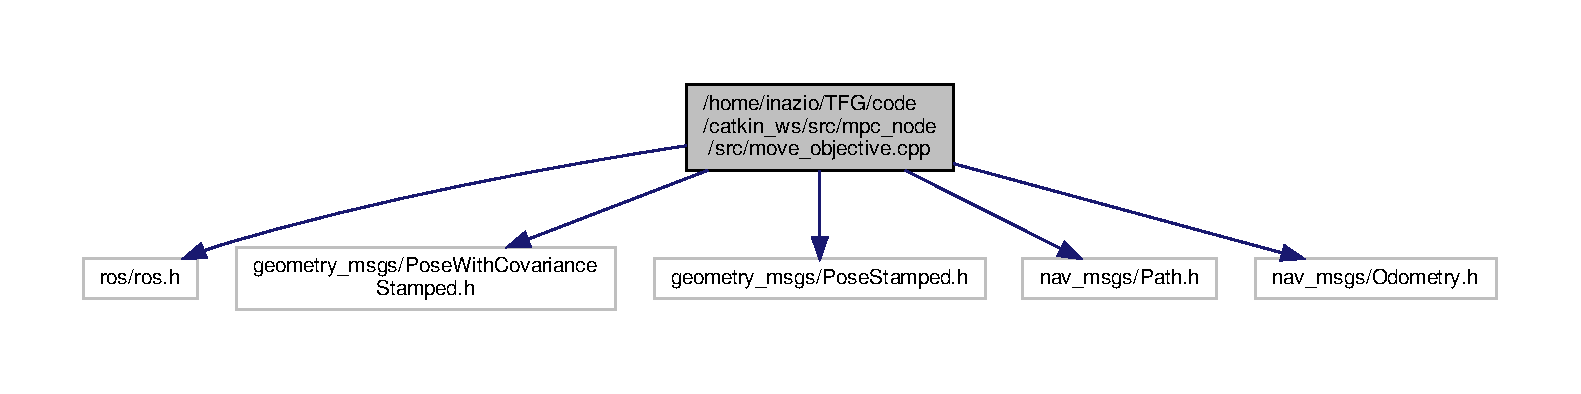
\includegraphics[width=350pt]{move__objective_8cpp__incl}
\end{center}
\end{figure}
\subsection*{Functions}
\begin{DoxyCompactItemize}
\item 
void \hyperlink{move__objective_8cpp_a40c3dca673fc26211e4101fd19240f7d}{publish\+\_\+obj\+\_\+actions} ()
\item 
int \hyperlink{move__objective_8cpp_a3c04138a5bfe5d72780bb7e82a18e627}{main} (int argc, char $\ast$$\ast$argv)
\end{DoxyCompactItemize}
\subsection*{Variables}
\begin{DoxyCompactItemize}
\item 
ros\+::\+Publisher \hyperlink{move__objective_8cpp_a4eae3dccc244c01bc93e0d6a05a05ce3}{pub\+V\+\_\+objetivo}
\item 
int \hyperlink{move__objective_8cpp_a2917b1dcf6f793ddef754e4b95a55cfa}{t\+\_\+objetivo}
\end{DoxyCompactItemize}


\subsection{Function Documentation}
\mbox{\Hypertarget{move__objective_8cpp_a3c04138a5bfe5d72780bb7e82a18e627}\label{move__objective_8cpp_a3c04138a5bfe5d72780bb7e82a18e627}} 
\index{move\+\_\+objective.\+cpp@{move\+\_\+objective.\+cpp}!main@{main}}
\index{main@{main}!move\+\_\+objective.\+cpp@{move\+\_\+objective.\+cpp}}
\subsubsection{\texorpdfstring{main()}{main()}}
{\footnotesize\ttfamily int main (\begin{DoxyParamCaption}\item[{int}]{argc,  }\item[{char $\ast$$\ast$}]{argv }\end{DoxyParamCaption})}

\mbox{\Hypertarget{move__objective_8cpp_a40c3dca673fc26211e4101fd19240f7d}\label{move__objective_8cpp_a40c3dca673fc26211e4101fd19240f7d}} 
\index{move\+\_\+objective.\+cpp@{move\+\_\+objective.\+cpp}!publish\+\_\+obj\+\_\+actions@{publish\+\_\+obj\+\_\+actions}}
\index{publish\+\_\+obj\+\_\+actions@{publish\+\_\+obj\+\_\+actions}!move\+\_\+objective.\+cpp@{move\+\_\+objective.\+cpp}}
\subsubsection{\texorpdfstring{publish\+\_\+obj\+\_\+actions()}{publish\_obj\_actions()}}
{\footnotesize\ttfamily void publish\+\_\+obj\+\_\+actions (\begin{DoxyParamCaption}{ }\end{DoxyParamCaption})}



\subsection{Variable Documentation}
\mbox{\Hypertarget{move__objective_8cpp_a4eae3dccc244c01bc93e0d6a05a05ce3}\label{move__objective_8cpp_a4eae3dccc244c01bc93e0d6a05a05ce3}} 
\index{move\+\_\+objective.\+cpp@{move\+\_\+objective.\+cpp}!pub\+V\+\_\+objetivo@{pub\+V\+\_\+objetivo}}
\index{pub\+V\+\_\+objetivo@{pub\+V\+\_\+objetivo}!move\+\_\+objective.\+cpp@{move\+\_\+objective.\+cpp}}
\subsubsection{\texorpdfstring{pub\+V\+\_\+objetivo}{pubV\_objetivo}}
{\footnotesize\ttfamily ros\+::\+Publisher pub\+V\+\_\+objetivo}

\mbox{\Hypertarget{move__objective_8cpp_a2917b1dcf6f793ddef754e4b95a55cfa}\label{move__objective_8cpp_a2917b1dcf6f793ddef754e4b95a55cfa}} 
\index{move\+\_\+objective.\+cpp@{move\+\_\+objective.\+cpp}!t\+\_\+objetivo@{t\+\_\+objetivo}}
\index{t\+\_\+objetivo@{t\+\_\+objetivo}!move\+\_\+objective.\+cpp@{move\+\_\+objective.\+cpp}}
\subsubsection{\texorpdfstring{t\+\_\+objetivo}{t\_objetivo}}
{\footnotesize\ttfamily int t\+\_\+objetivo}


\hypertarget{MPC__main_8cpp}{}\section{/home/inazio/\+T\+F\+G/code/catkin\+\_\+ws/src/mpc\+\_\+node/src/\+M\+P\+C\+\_\+main.cpp File Reference}
\label{MPC__main_8cpp}\index{/home/inazio/\+T\+F\+G/code/catkin\+\_\+ws/src/mpc\+\_\+node/src/\+M\+P\+C\+\_\+main.\+cpp@{/home/inazio/\+T\+F\+G/code/catkin\+\_\+ws/src/mpc\+\_\+node/src/\+M\+P\+C\+\_\+main.\+cpp}}
{\ttfamily \#include \char`\"{}mpc\+\_\+node.\+cpp\char`\"{}}\newline
{\ttfamily \#include \char`\"{}ros/ros.\+h\char`\"{}}\newline
Include dependency graph for M\+P\+C\+\_\+main.\+cpp\+:\nopagebreak
\begin{figure}[H]
\begin{center}
\leavevmode
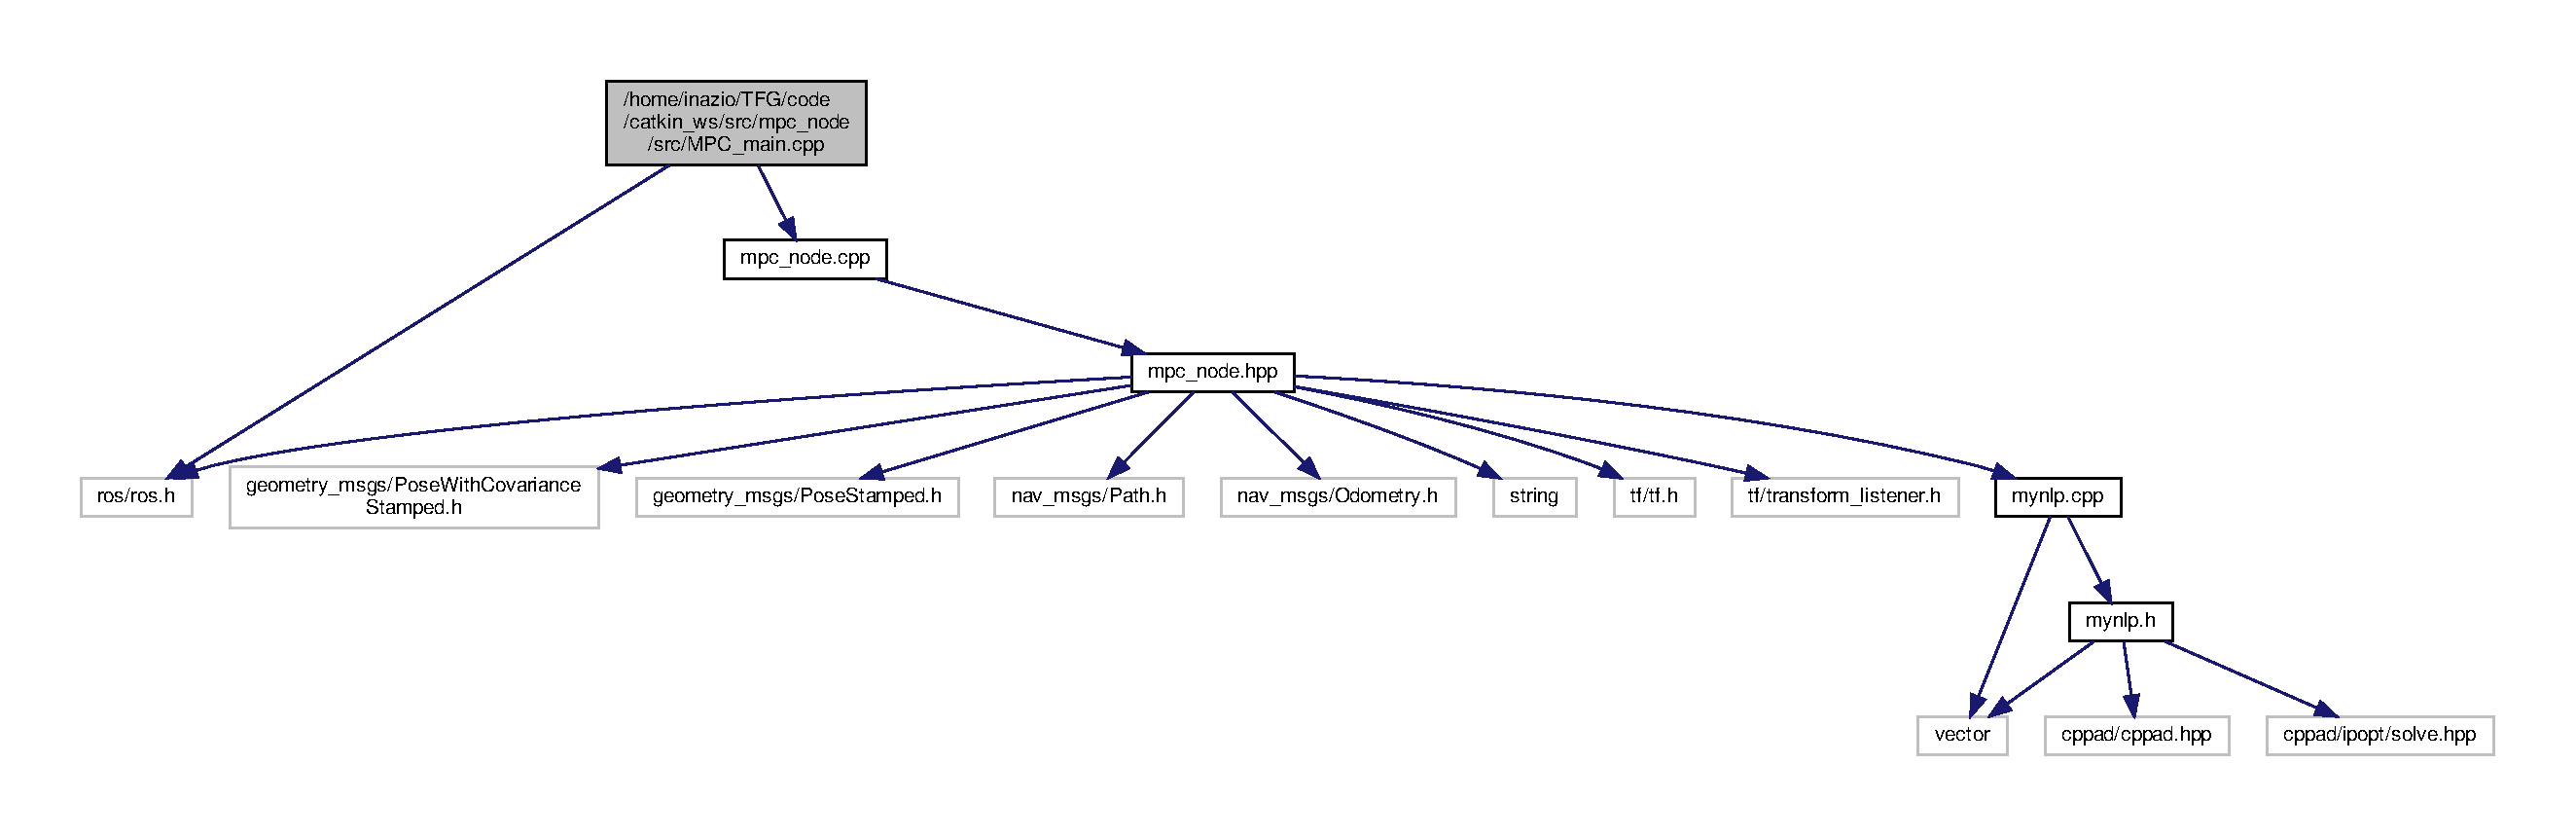
\includegraphics[width=350pt]{MPC__main_8cpp__incl}
\end{center}
\end{figure}
\subsection*{Functions}
\begin{DoxyCompactItemize}
\item 
int \hyperlink{MPC__main_8cpp_a3c04138a5bfe5d72780bb7e82a18e627}{main} (int argc, char $\ast$$\ast$argv)
\end{DoxyCompactItemize}


\subsection{Function Documentation}
\mbox{\Hypertarget{MPC__main_8cpp_a3c04138a5bfe5d72780bb7e82a18e627}\label{MPC__main_8cpp_a3c04138a5bfe5d72780bb7e82a18e627}} 
\index{M\+P\+C\+\_\+main.\+cpp@{M\+P\+C\+\_\+main.\+cpp}!main@{main}}
\index{main@{main}!M\+P\+C\+\_\+main.\+cpp@{M\+P\+C\+\_\+main.\+cpp}}
\subsubsection{\texorpdfstring{main()}{main()}}
{\footnotesize\ttfamily int main (\begin{DoxyParamCaption}\item[{int}]{argc,  }\item[{char $\ast$$\ast$}]{argv }\end{DoxyParamCaption})}


\hypertarget{mpc__node_8cpp}{}\section{/home/inazio/\+T\+F\+G/code/catkin\+\_\+ws/src/mpc\+\_\+node/src/mpc\+\_\+node.cpp File Reference}
\label{mpc__node_8cpp}\index{/home/inazio/\+T\+F\+G/code/catkin\+\_\+ws/src/mpc\+\_\+node/src/mpc\+\_\+node.\+cpp@{/home/inazio/\+T\+F\+G/code/catkin\+\_\+ws/src/mpc\+\_\+node/src/mpc\+\_\+node.\+cpp}}
{\ttfamily \#include \char`\"{}mpc\+\_\+node.\+hpp\char`\"{}}\newline
Include dependency graph for mpc\+\_\+node.\+cpp\+:\nopagebreak
\begin{figure}[H]
\begin{center}
\leavevmode
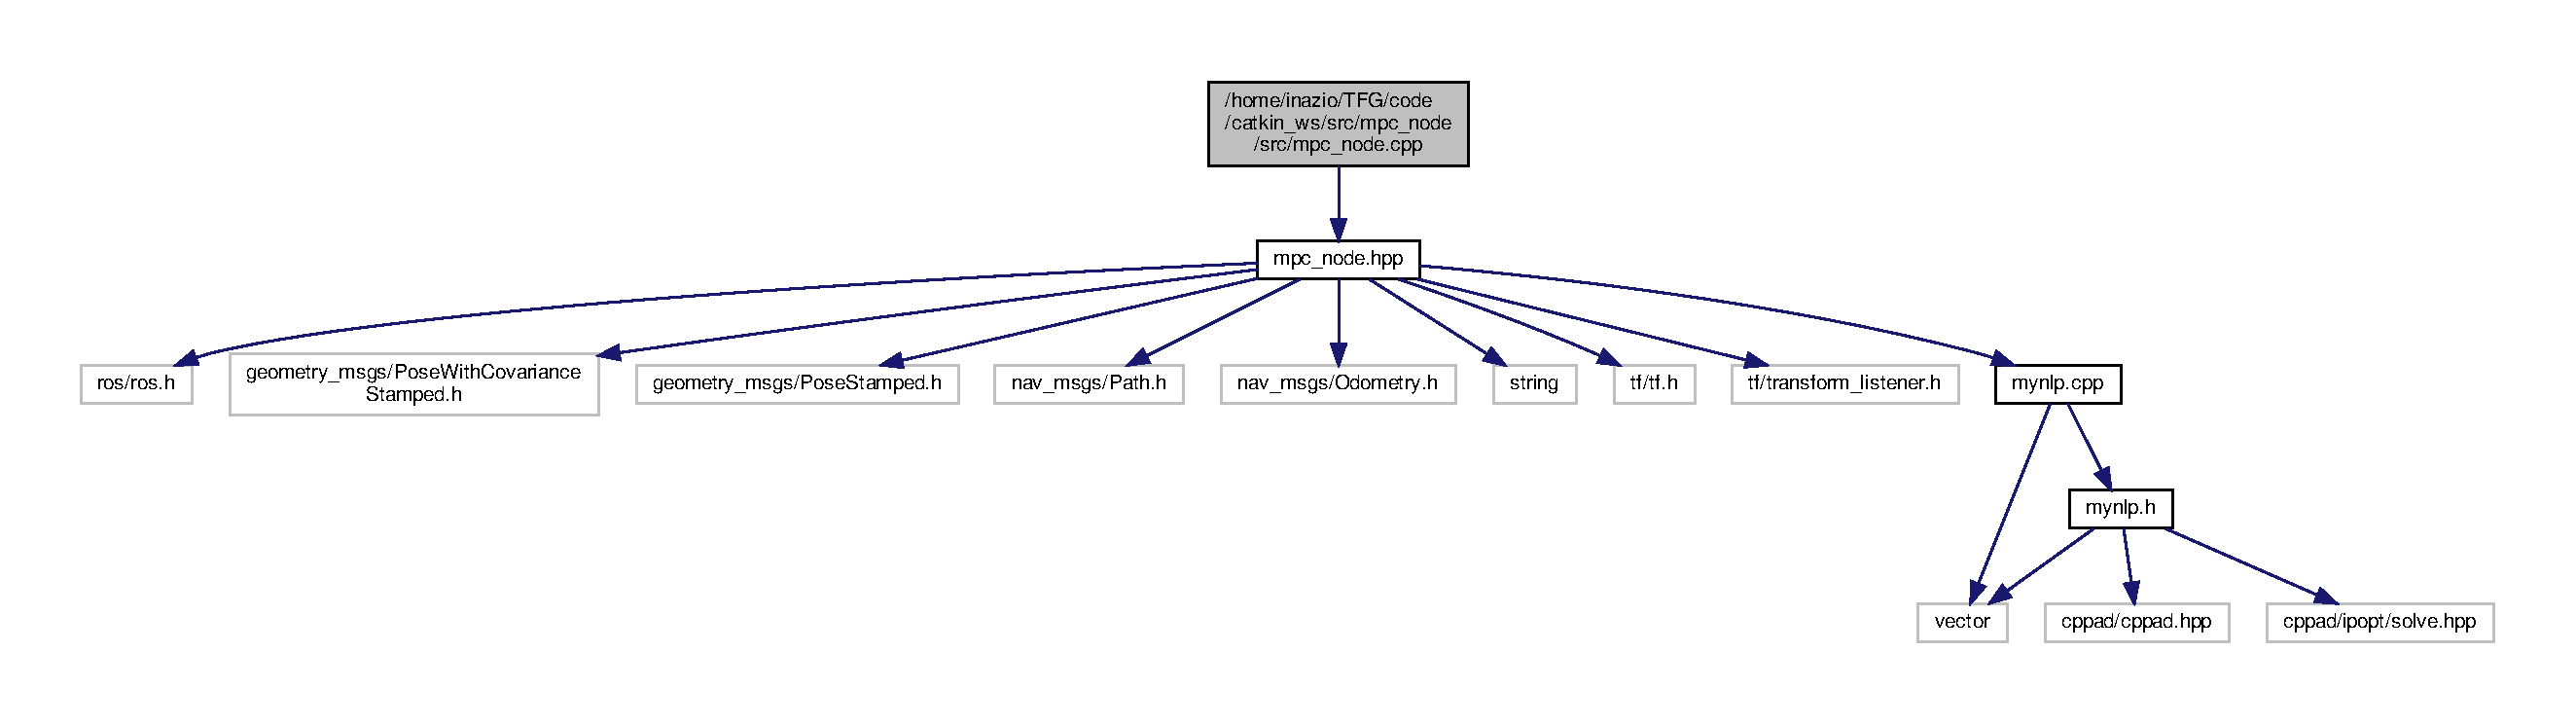
\includegraphics[width=350pt]{mpc__node_8cpp__incl}
\end{center}
\end{figure}
This graph shows which files directly or indirectly include this file\+:\nopagebreak
\begin{figure}[H]
\begin{center}
\leavevmode
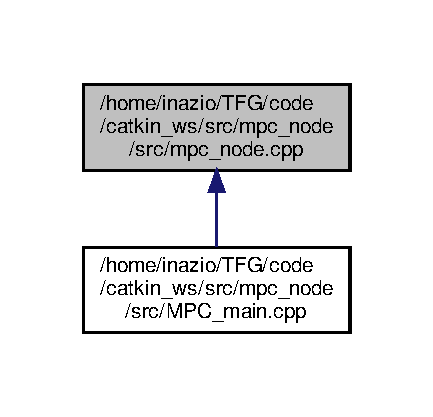
\includegraphics[width=208pt]{mpc__node_8cpp__dep__incl}
\end{center}
\end{figure}

\hypertarget{mpc__node_8hpp}{}\section{/home/inazio/\+T\+F\+G/code/catkin\+\_\+ws/src/mpc\+\_\+node/src/mpc\+\_\+node.hpp File Reference}
\label{mpc__node_8hpp}\index{/home/inazio/\+T\+F\+G/code/catkin\+\_\+ws/src/mpc\+\_\+node/src/mpc\+\_\+node.\+hpp@{/home/inazio/\+T\+F\+G/code/catkin\+\_\+ws/src/mpc\+\_\+node/src/mpc\+\_\+node.\+hpp}}
{\ttfamily \#include \char`\"{}ros/ros.\+h\char`\"{}}\newline
{\ttfamily \#include $<$geometry\+\_\+msgs/\+Pose\+With\+Covariance\+Stamped.\+h$>$}\newline
{\ttfamily \#include $<$geometry\+\_\+msgs/\+Pose\+Stamped.\+h$>$}\newline
{\ttfamily \#include $<$nav\+\_\+msgs/\+Path.\+h$>$}\newline
{\ttfamily \#include $<$nav\+\_\+msgs/\+Odometry.\+h$>$}\newline
{\ttfamily \#include $<$string$>$}\newline
{\ttfamily \#include $<$tf/tf.\+h$>$}\newline
{\ttfamily \#include $<$tf/transform\+\_\+listener.\+h$>$}\newline
{\ttfamily \#include \char`\"{}mynlp.\+cpp\char`\"{}}\newline
Include dependency graph for mpc\+\_\+node.\+hpp\+:\nopagebreak
\begin{figure}[H]
\begin{center}
\leavevmode
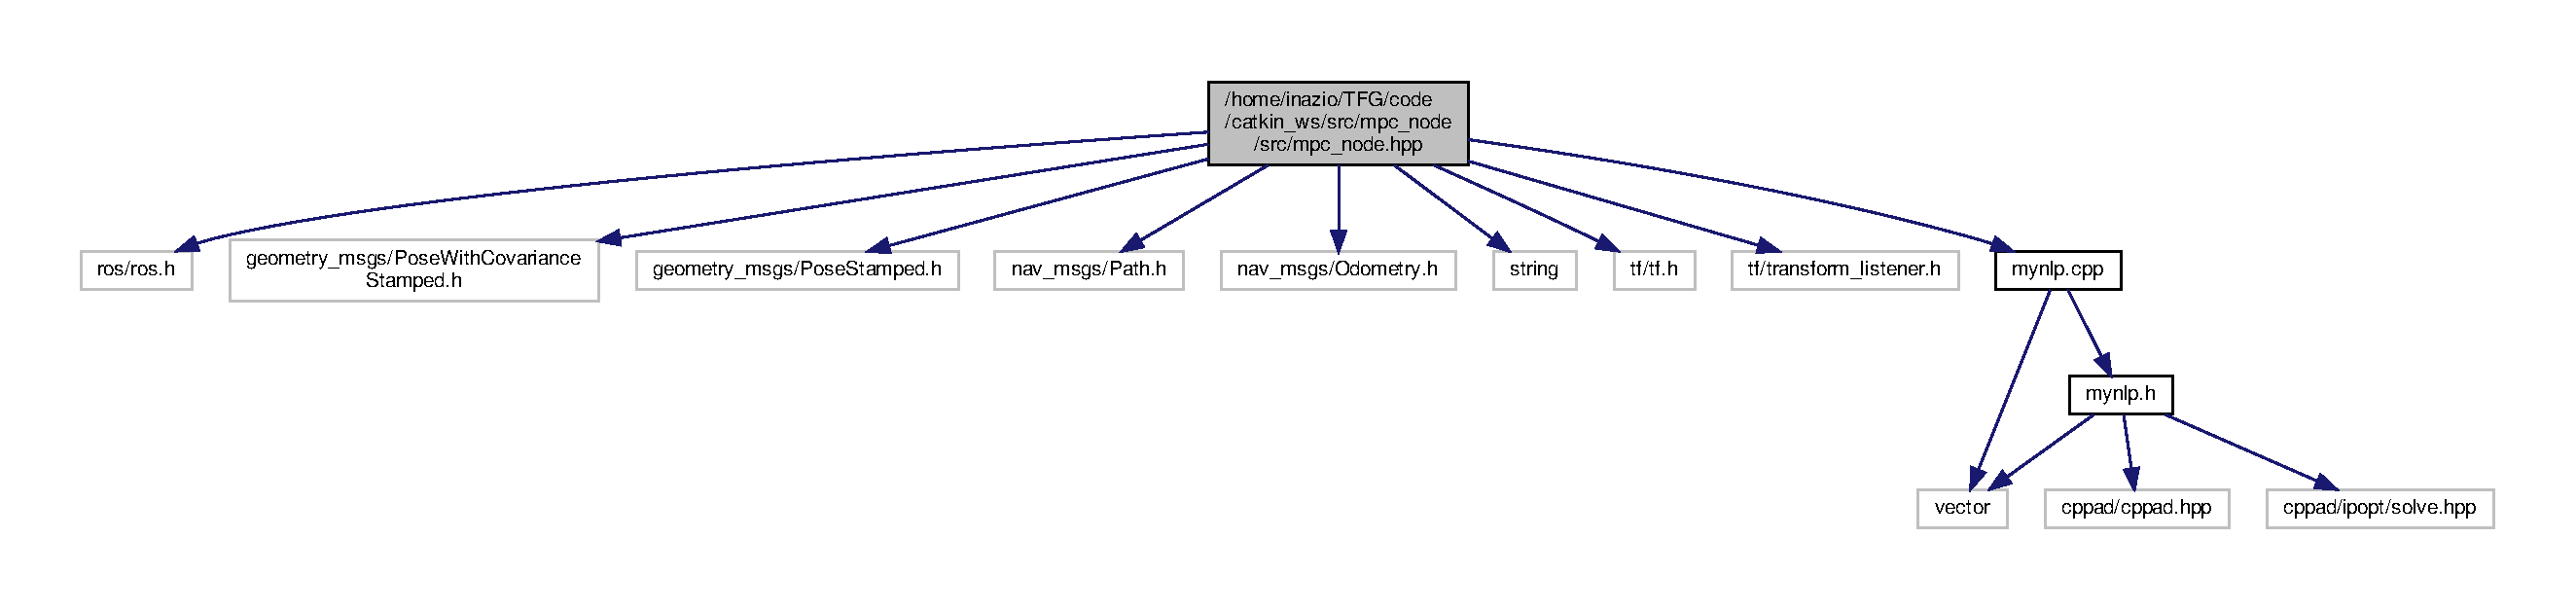
\includegraphics[width=350pt]{mpc__node_8hpp__incl}
\end{center}
\end{figure}
This graph shows which files directly or indirectly include this file\+:\nopagebreak
\begin{figure}[H]
\begin{center}
\leavevmode
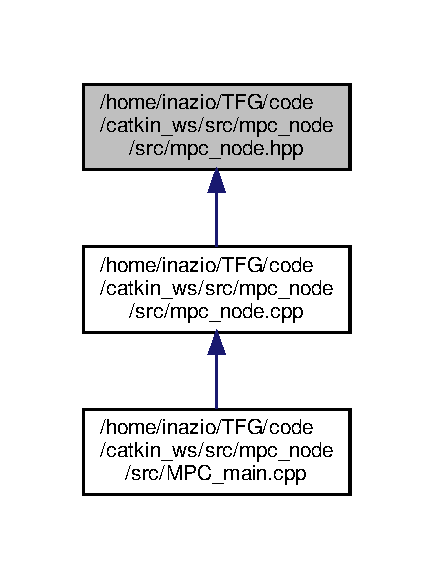
\includegraphics[width=208pt]{mpc__node_8hpp__dep__incl}
\end{center}
\end{figure}
\subsection*{Classes}
\begin{DoxyCompactItemize}
\item 
class \hyperlink{classMpc__node}{Mpc\+\_\+node}
\end{DoxyCompactItemize}

\hypertarget{mynlp_8cpp}{}\section{/home/inazio/\+T\+F\+G/code/catkin\+\_\+ws/src/mpc\+\_\+node/src/mynlp.cpp File Reference}
\label{mynlp_8cpp}\index{/home/inazio/\+T\+F\+G/code/catkin\+\_\+ws/src/mpc\+\_\+node/src/mynlp.\+cpp@{/home/inazio/\+T\+F\+G/code/catkin\+\_\+ws/src/mpc\+\_\+node/src/mynlp.\+cpp}}
{\ttfamily \#include \char`\"{}mynlp.\+h\char`\"{}}\newline
{\ttfamily \#include $<$vector$>$}\newline
Include dependency graph for mynlp.\+cpp\+:\nopagebreak
\begin{figure}[H]
\begin{center}
\leavevmode
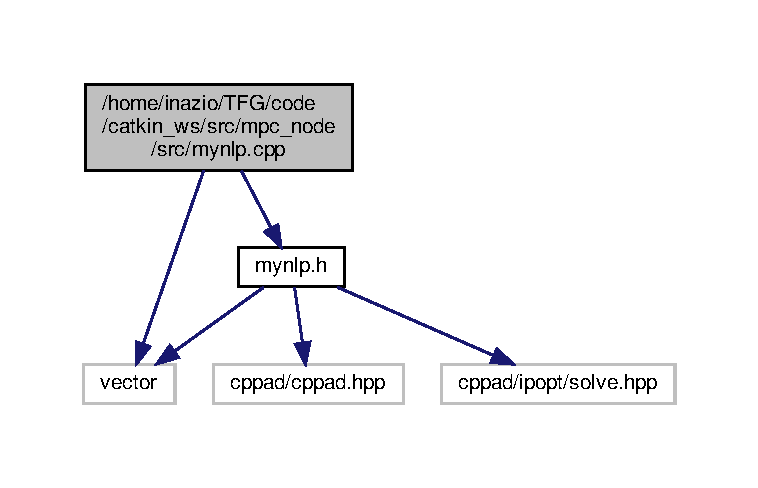
\includegraphics[width=350pt]{mynlp_8cpp__incl}
\end{center}
\end{figure}
This graph shows which files directly or indirectly include this file\+:\nopagebreak
\begin{figure}[H]
\begin{center}
\leavevmode
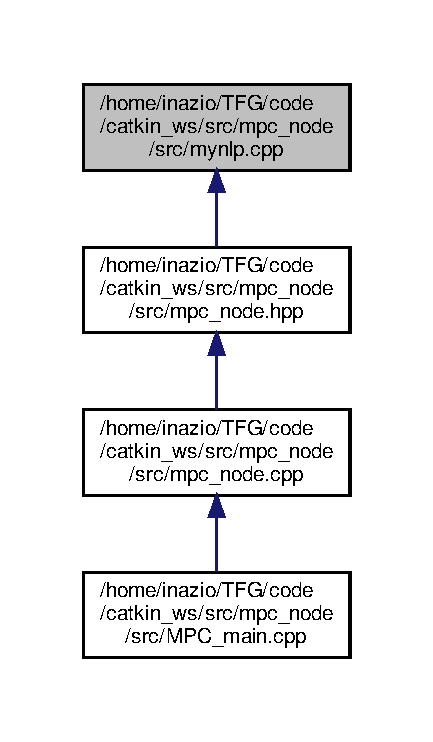
\includegraphics[width=208pt]{mynlp_8cpp__dep__incl}
\end{center}
\end{figure}
\subsection*{Variables}
\begin{DoxyCompactItemize}
\item 
size\+\_\+t \hyperlink{mynlp_8cpp_aa6d2142329b3b553ce8a778f8239db33}{N} = 10
\item 
AD$<$ double $>$ \hyperlink{mynlp_8cpp_a6cb95d1842dea8d8a0ebcf523d9451be}{dt} = 0.\+1
\item 
size\+\_\+t \hyperlink{mynlp_8cpp_a3a8a508bade6ce1fe8d51efa0b4b1c13}{x\+\_\+start} = 0
\item 
size\+\_\+t \hyperlink{mynlp_8cpp_ab248b1e39ab3bea19bef732655e68902}{y\+\_\+start} = \hyperlink{mynlp_8cpp_a3a8a508bade6ce1fe8d51efa0b4b1c13}{x\+\_\+start} + \hyperlink{mynlp_8cpp_aa6d2142329b3b553ce8a778f8239db33}{N}
\item 
size\+\_\+t \hyperlink{mynlp_8cpp_a1e08221d514968bda0e872228f3e07fa}{tita\+\_\+start} = \hyperlink{mynlp_8cpp_ab248b1e39ab3bea19bef732655e68902}{y\+\_\+start} + \hyperlink{mynlp_8cpp_aa6d2142329b3b553ce8a778f8239db33}{N}
\item 
size\+\_\+t \hyperlink{mynlp_8cpp_ab813308047cbabde1b1fc4e86c76922f}{V\+\_\+start} = \hyperlink{mynlp_8cpp_a1e08221d514968bda0e872228f3e07fa}{tita\+\_\+start} + \hyperlink{mynlp_8cpp_aa6d2142329b3b553ce8a778f8239db33}{N}
\item 
size\+\_\+t \hyperlink{mynlp_8cpp_ad1330d9c6590d7dd45d69276e2e6c58c}{W\+\_\+start} = \hyperlink{mynlp_8cpp_ab813308047cbabde1b1fc4e86c76922f}{V\+\_\+start} + \hyperlink{mynlp_8cpp_aa6d2142329b3b553ce8a778f8239db33}{N}-\/1
\end{DoxyCompactItemize}


\subsection{Variable Documentation}
\mbox{\Hypertarget{mynlp_8cpp_a6cb95d1842dea8d8a0ebcf523d9451be}\label{mynlp_8cpp_a6cb95d1842dea8d8a0ebcf523d9451be}} 
\index{mynlp.\+cpp@{mynlp.\+cpp}!dt@{dt}}
\index{dt@{dt}!mynlp.\+cpp@{mynlp.\+cpp}}
\subsubsection{\texorpdfstring{dt}{dt}}
{\footnotesize\ttfamily AD$<$double$>$ dt = 0.\+1}

\mbox{\Hypertarget{mynlp_8cpp_aa6d2142329b3b553ce8a778f8239db33}\label{mynlp_8cpp_aa6d2142329b3b553ce8a778f8239db33}} 
\index{mynlp.\+cpp@{mynlp.\+cpp}!N@{N}}
\index{N@{N}!mynlp.\+cpp@{mynlp.\+cpp}}
\subsubsection{\texorpdfstring{N}{N}}
{\footnotesize\ttfamily size\+\_\+t N = 10}

\mbox{\Hypertarget{mynlp_8cpp_a1e08221d514968bda0e872228f3e07fa}\label{mynlp_8cpp_a1e08221d514968bda0e872228f3e07fa}} 
\index{mynlp.\+cpp@{mynlp.\+cpp}!tita\+\_\+start@{tita\+\_\+start}}
\index{tita\+\_\+start@{tita\+\_\+start}!mynlp.\+cpp@{mynlp.\+cpp}}
\subsubsection{\texorpdfstring{tita\+\_\+start}{tita\_start}}
{\footnotesize\ttfamily size\+\_\+t tita\+\_\+start = \hyperlink{mynlp_8cpp_ab248b1e39ab3bea19bef732655e68902}{y\+\_\+start} + \hyperlink{mynlp_8cpp_aa6d2142329b3b553ce8a778f8239db33}{N}}

\mbox{\Hypertarget{mynlp_8cpp_ab813308047cbabde1b1fc4e86c76922f}\label{mynlp_8cpp_ab813308047cbabde1b1fc4e86c76922f}} 
\index{mynlp.\+cpp@{mynlp.\+cpp}!V\+\_\+start@{V\+\_\+start}}
\index{V\+\_\+start@{V\+\_\+start}!mynlp.\+cpp@{mynlp.\+cpp}}
\subsubsection{\texorpdfstring{V\+\_\+start}{V\_start}}
{\footnotesize\ttfamily size\+\_\+t V\+\_\+start = \hyperlink{mynlp_8cpp_a1e08221d514968bda0e872228f3e07fa}{tita\+\_\+start} + \hyperlink{mynlp_8cpp_aa6d2142329b3b553ce8a778f8239db33}{N}}

\mbox{\Hypertarget{mynlp_8cpp_ad1330d9c6590d7dd45d69276e2e6c58c}\label{mynlp_8cpp_ad1330d9c6590d7dd45d69276e2e6c58c}} 
\index{mynlp.\+cpp@{mynlp.\+cpp}!W\+\_\+start@{W\+\_\+start}}
\index{W\+\_\+start@{W\+\_\+start}!mynlp.\+cpp@{mynlp.\+cpp}}
\subsubsection{\texorpdfstring{W\+\_\+start}{W\_start}}
{\footnotesize\ttfamily size\+\_\+t W\+\_\+start = \hyperlink{mynlp_8cpp_ab813308047cbabde1b1fc4e86c76922f}{V\+\_\+start} + \hyperlink{mynlp_8cpp_aa6d2142329b3b553ce8a778f8239db33}{N}-\/1}

\mbox{\Hypertarget{mynlp_8cpp_a3a8a508bade6ce1fe8d51efa0b4b1c13}\label{mynlp_8cpp_a3a8a508bade6ce1fe8d51efa0b4b1c13}} 
\index{mynlp.\+cpp@{mynlp.\+cpp}!x\+\_\+start@{x\+\_\+start}}
\index{x\+\_\+start@{x\+\_\+start}!mynlp.\+cpp@{mynlp.\+cpp}}
\subsubsection{\texorpdfstring{x\+\_\+start}{x\_start}}
{\footnotesize\ttfamily size\+\_\+t x\+\_\+start = 0}

\mbox{\Hypertarget{mynlp_8cpp_ab248b1e39ab3bea19bef732655e68902}\label{mynlp_8cpp_ab248b1e39ab3bea19bef732655e68902}} 
\index{mynlp.\+cpp@{mynlp.\+cpp}!y\+\_\+start@{y\+\_\+start}}
\index{y\+\_\+start@{y\+\_\+start}!mynlp.\+cpp@{mynlp.\+cpp}}
\subsubsection{\texorpdfstring{y\+\_\+start}{y\_start}}
{\footnotesize\ttfamily size\+\_\+t y\+\_\+start = \hyperlink{mynlp_8cpp_a3a8a508bade6ce1fe8d51efa0b4b1c13}{x\+\_\+start} + \hyperlink{mynlp_8cpp_aa6d2142329b3b553ce8a778f8239db33}{N}}


\hypertarget{mynlp_8h}{}\section{/home/inazio/\+T\+F\+G/code/catkin\+\_\+ws/src/mpc\+\_\+node/src/mynlp.h File Reference}
\label{mynlp_8h}\index{/home/inazio/\+T\+F\+G/code/catkin\+\_\+ws/src/mpc\+\_\+node/src/mynlp.\+h@{/home/inazio/\+T\+F\+G/code/catkin\+\_\+ws/src/mpc\+\_\+node/src/mynlp.\+h}}
{\ttfamily \#include $<$vector$>$}\newline
{\ttfamily \#include $<$cppad/cppad.\+hpp$>$}\newline
{\ttfamily \#include $<$cppad/ipopt/solve.\+hpp$>$}\newline
Include dependency graph for mynlp.\+h\+:\nopagebreak
\begin{figure}[H]
\begin{center}
\leavevmode
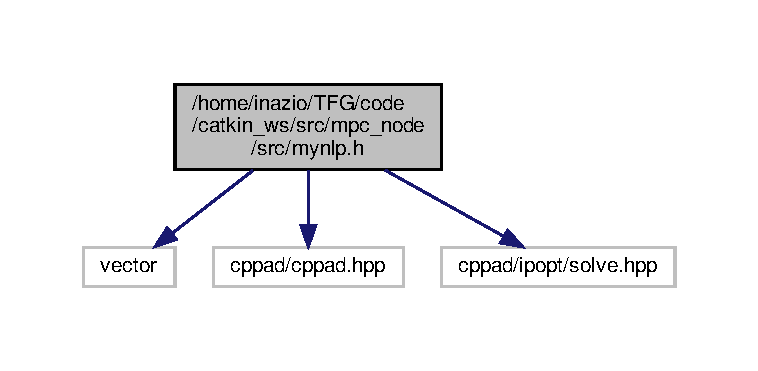
\includegraphics[width=350pt]{mynlp_8h__incl}
\end{center}
\end{figure}
This graph shows which files directly or indirectly include this file\+:\nopagebreak
\begin{figure}[H]
\begin{center}
\leavevmode
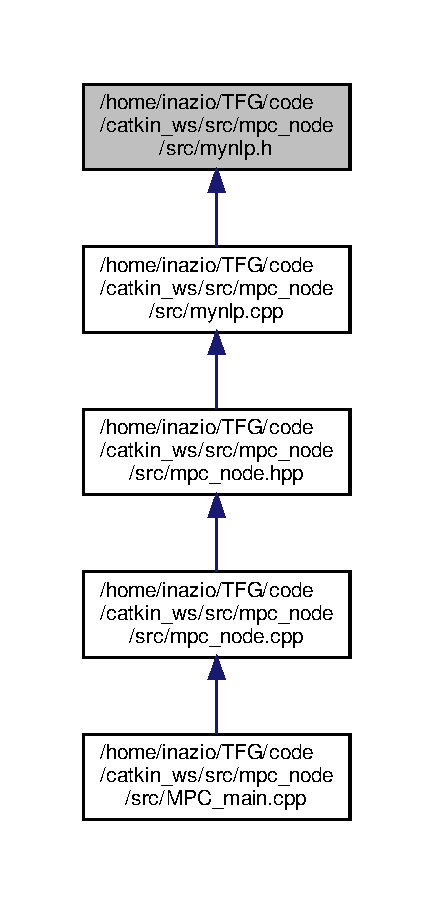
\includegraphics[width=208pt]{mynlp_8h__dep__incl}
\end{center}
\end{figure}
\subsection*{Classes}
\begin{DoxyCompactItemize}
\item 
class \hyperlink{classFG__eval}{F\+G\+\_\+eval}
\item 
class \hyperlink{classmyNLP}{my\+N\+LP}
\end{DoxyCompactItemize}
\subsection*{Macros}
\begin{DoxyCompactItemize}
\item 
\#define \hyperlink{mynlp_8h_a58ba52a422b8a08f76f517637242369b}{F\+G\+\_\+\+E\+V\+A\+L\+\_\+H}
\item 
\#define \hyperlink{mynlp_8h_ae4b1ab2fd1598e634c0d319125790f8f}{M\+Y\+N\+L\+P\+\_\+H}
\end{DoxyCompactItemize}
\subsection*{Functions}
\begin{DoxyCompactItemize}
\item 
typedef \hyperlink{mynlp_8h_a9b5b39b87fcb971c45e44b1be300ad5e}{C\+P\+P\+A\+D\+\_\+\+T\+E\+S\+T\+V\+E\+C\+T\+OR} (double) Dvector
\end{DoxyCompactItemize}


\subsection{Macro Definition Documentation}
\mbox{\Hypertarget{mynlp_8h_a58ba52a422b8a08f76f517637242369b}\label{mynlp_8h_a58ba52a422b8a08f76f517637242369b}} 
\index{mynlp.\+h@{mynlp.\+h}!F\+G\+\_\+\+E\+V\+A\+L\+\_\+H@{F\+G\+\_\+\+E\+V\+A\+L\+\_\+H}}
\index{F\+G\+\_\+\+E\+V\+A\+L\+\_\+H@{F\+G\+\_\+\+E\+V\+A\+L\+\_\+H}!mynlp.\+h@{mynlp.\+h}}
\subsubsection{\texorpdfstring{F\+G\+\_\+\+E\+V\+A\+L\+\_\+H}{FG\_EVAL\_H}}
{\footnotesize\ttfamily \#define F\+G\+\_\+\+E\+V\+A\+L\+\_\+H}

\mbox{\Hypertarget{mynlp_8h_ae4b1ab2fd1598e634c0d319125790f8f}\label{mynlp_8h_ae4b1ab2fd1598e634c0d319125790f8f}} 
\index{mynlp.\+h@{mynlp.\+h}!M\+Y\+N\+L\+P\+\_\+H@{M\+Y\+N\+L\+P\+\_\+H}}
\index{M\+Y\+N\+L\+P\+\_\+H@{M\+Y\+N\+L\+P\+\_\+H}!mynlp.\+h@{mynlp.\+h}}
\subsubsection{\texorpdfstring{M\+Y\+N\+L\+P\+\_\+H}{MYNLP\_H}}
{\footnotesize\ttfamily \#define M\+Y\+N\+L\+P\+\_\+H}



\subsection{Function Documentation}
\mbox{\Hypertarget{mynlp_8h_a9b5b39b87fcb971c45e44b1be300ad5e}\label{mynlp_8h_a9b5b39b87fcb971c45e44b1be300ad5e}} 
\index{mynlp.\+h@{mynlp.\+h}!C\+P\+P\+A\+D\+\_\+\+T\+E\+S\+T\+V\+E\+C\+T\+OR@{C\+P\+P\+A\+D\+\_\+\+T\+E\+S\+T\+V\+E\+C\+T\+OR}}
\index{C\+P\+P\+A\+D\+\_\+\+T\+E\+S\+T\+V\+E\+C\+T\+OR@{C\+P\+P\+A\+D\+\_\+\+T\+E\+S\+T\+V\+E\+C\+T\+OR}!mynlp.\+h@{mynlp.\+h}}
\subsubsection{\texorpdfstring{C\+P\+P\+A\+D\+\_\+\+T\+E\+S\+T\+V\+E\+C\+T\+O\+R()}{CPPAD\_TESTVECTOR()}}
{\footnotesize\ttfamily typedef C\+P\+P\+A\+D\+\_\+\+T\+E\+S\+T\+V\+E\+C\+T\+OR (\begin{DoxyParamCaption}\item[{double}]{ }\end{DoxyParamCaption})}


%--- End generated contents ---

% Index
\backmatter
\newpage
\phantomsection
\clearemptydoublepage
\addcontentsline{toc}{chapter}{Index}
\printindex

\end{document}
